\documentclass{report}
%\usepackage{fullpage}

\usepackage[top=1in, bottom=1in, left=1.25in, right=.75in]{geometry}

    \usepackage{fancyhdr}
    \pagestyle{fancy}
    \lhead{PSD 2.0}
    \chead{}
    \rhead{\fancyplain{}{\textit{\leftmark}}}
 
 \usepackage[LGR,T1]{fontenc}
 
%\renewcommand{\familydefault}{\sfdefault}
%\usepackage[scaled=1]{helvet}
%\usepackage[helvet]{sfmath}
%\everymath={\sf}

\usepackage{parskip}
\usepackage[colorinlistoftodos]{todonotes}
\usepackage[colorlinks=true, allcolors=blue]{hyperref}

\usepackage{amsmath}
\usepackage{amsfonts}
\usepackage{amssymb}
\usepackage{bbm}
\usepackage{bm}
\usepackage{cleveref}
\usepackage{listings}
\usepackage{graphbox,graphicx}
\usepackage{siunitx}
\usepackage{subcaption}
\usepackage{textcomp}
\usepackage{babel}
\usepackage[autostyle=false]{csquotes}


\usepackage{stmaryrd}
\usepackage{xcolor}
\definecolor{halfgray}{gray}{0.55}
\definecolor{ipython_frame}{RGB}{207, 207, 207}

\usepackage{color}
\definecolor{eclipseBlue}{RGB}{42,0.0,255}
\definecolor{eclipseGreen}{RGB}{63,127,95}
\definecolor{eclipsePurple}{RGB}{127,0,85}



\lstdefinelanguage{iPython}{
    commentstyle=\color{cyan}\ttfamily,
    stringstyle=\color{red}\ttfamily,
    keepspaces=true,
    showspaces=false,
    showstringspaces=false,
    %
    rulecolor=\color{ipython_frame},
    frame=single,
    frameround={t}{t}{t}{t},
    framexleftmargin=6mm,
    numbers=left,
    numberstyle=\tiny\color{halfgray},
    %
    basicstyle=\scriptsize\ttfamily,
    keywordstyle=\color{green}\ttfamily,
}

\lstdefinelanguage{PSD}
{
  % list of keywords
  morekeywords={
    import,
    if,
    while,
    for,
    np
  },
  sensitive=false, % keywords are not case-sensitive
  morecomment=[l]{//}, % l is for line comment
  morecomment=[s]{/*}{*/}, % s is for start and end delimiter
  morestring=[b]" % defines that strings are enclosed in double quotes
}

\lstdefinestyle{Linux}
{
 backgroundcolor=\color{white},
 basicstyle=\scriptsize\color{black}\ttfamily,
    frame=trbl, % draw a frame at the top, right, left and bottom of the listing
  frameround=tttt, % make the frame round at all four corners
  framesep=4pt, % quarter circle size of the round corners
}

\DeclareRobustCommand{\greektext}{%
  \fontencoding{LGR}\selectfont\def\encodingdefault{LGR}}
\DeclareRobustCommand{\textgreek}[1]{\leavevmode{\greektext #1}}
\ProvideTextCommand{\~}{LGR}[1]{\char126#1}

\newcommand{\assemble}{%
  \mathop{\vcenter{\hbox{\Large\bfseries \textsf{A}}}}\displaylimits}
  
%%%%%%%%%%%%%%%%%%%%%%%%%%%%%%%%%%  NEW COMMANDS %%%%%%%%%%%%%%%%%%%%%%%%%%%%%%%%%%
\newcommand{\bA}{\textbf{A}}
\newcommand{\bM}{\textbf{M}} 
\newcommand{\bx}{\textbf{x}} 
\newcommand{\bb}{\textbf{b}} 
\newcommand{\br}{\textbf{r}}
\newcommand{\bu}{\textbf{u}}
\newcommand{\bv}{\textbf{v}}
\newcommand{\bt}{\boldsymbol t}
\newcommand{\bl}{\boldsymbol f}
\newcommand{\bnv}{N_{\text{v}}}
\newcommand{\bnd}{N_{\text{DOF}}}
\newcommand{\bnz}{N_{\text{nz}}}
\newcommand{\bgc}{G_{\text{c}}}
\newcommand{\buh}{\boldsymbol u^h}
\newcommand{\bvh}{\boldsymbol v^h}
\newcommand{\bwh}{\boldsymbol w^h}
\newcommand{\bqh}{\boldsymbol q^h}
\newcommand{\bz}{\textbf{z}}
\newcommand{\bp}{\textbf{p}}
\newcommand{\np}{N_\text{p}}
\newcommand{\wu}{\widehat{u}}
\newcommand{\wbu}{\widehat{\textbf{u}}}
\newcommand{\we}{\widehat{\varepsilon}}
\newcommand{\ws}{\widehat{\sigma}}
\newcommand{\wf}{\widehat{f}}
\newcommand{\bff}{\textbf{f}}
\newcommand{\fih}{ d^h}
\newcommand{\ttah}{ \theta^h}
\newcommand{\sig}{\boldsymbol{\sigma}}
\newcommand{\eps}{\boldsymbol{\varepsilon}} 
\newcommand{\dv}{\mathrm{d}\text{v}}
\newcommand{\ds}{\mathrm{d}\text{s}}
%%%%%%%%%%%%%%%%%%%%%%%%%%%%%%%%%%%%%%%%%%%%%%%%%%%%%%%%%%%%%%%%%%%%%%%%%%%%%%%%%%%

\newcommand{\RR}{I\!\!R}
\newcommand{\NN}{I\!\!N}
\newcommand{\field}[1]{\mathbb{#1}}
\newcommand{\uu }[1]{\pmb{#1}}
\newcommand{\ten}[1]{\pmb{\mathbb{#1}}}
\newcommand{\sprod}{\underline{\otimes}}
\newcommand{\tr}{\mathop{\rm tr}}
\newcommand{\dd}{{\rm d}}
\renewcommand{\det}{\mathop{\rm det}}

\newcommand{\eul}{\mbox{e}}

\def\Tij{{T_{ij}}}

\def\bxi{\mbox{\boldmath${\xi}$}}
\def\balpha{\mbox{\boldmath${\alpha}$}}
\def\bepsilon{\mbox{\boldmath${\epsilon}$}}
%\def\bepsilon{\mbox{\boldmath$\underline{\underline{{\epsilon}}}$}}
\def\bkappa{\mbox{\boldmath${\kappa}$}}
\def\bphi{\mbox{\boldmath${\phi}$}}
\def\bsigma{\mbox{\boldmath${\sigma}$}}

\def\bA{{{\bf{A}}}}
\def\ba{{\bf{a}}}
\def\bB{{\bf B}}
\def\bb{{\bf{b}}}
\def\bC{{\bf C}}
\def\bc{{\bf c}}
\def\bd{{\bf d}}
\def\bD{{{\bf{D}}}}
\def\bE{{\bf E}}
\def\be{{\bf e}}
\def\be{{\bf{e}}}
\def\bF{{\bf F}}
\def\bfvec{{\bf{f}}}
\def\bG{{\bf G}}
\def\bI{{{\bf{I}}}}
\def\bg{{\bf{g}}}
\def\bh{{\bf h}}
\def\bi{{\bf i}}
\def\bH{{\bf H}}
\def\bk{{\bf k}}
\def\bK{{\bf K}}
\def\bl{{\bf l}}
\def\bL{{\bf L}}
\def\bM{{\bf M}}
\def\bN{{\bf N}}
\def\bn{{\bf{n}}}
\def\bm{{\bf m}}
\def\b0{{\bf 0}}
\def\b1{{\bf 1}}
\def\bo{{\bf o}}
\def\bX{{\bf X}}
\def\bZ{{\bf Z}}
\def\bx{{\bf{x}}}                   
\def\bP{{\bf P}}
\def\bp{{\bf p}}
\def\bQ{{\bf Q}}
\def\bq{{\bf q}}
\def\br{{\bf r}}
\def\bR{{\bf R}}
\def\bS{{\bf S}}
\def\bs{{\bf s}}
\def\bT{{\bf{T}}}
\def\bt{{\bf t}}
\def\bU{{\bf U}}
\def\bu{{\bf{u}}}
\def\bV{{\bf{V}}}                   
\def\bv{{\bf{v}}}
\def\bw{{\bf w}}
\def\bW{{\bf W}}
\def\vecbx{{\bf x}}
\def\by{{\bf y}}
\def\bY{{\bf Y}}
\def\bz{{\bf z}}
\def\bY{{\bf Y}}
\def\Id{{\bf 1}}


%\bibliography{biblio.bib}
\usepackage[style=numeric]{biblatex}
%\usepackage[citestyle=alphabetic,bibstyle=authortitle]{biblatex}

\addbibresource{biblio.bib}

\title{PSD}
\author{}
%\author{Mohd Afeef Badri,~Giuseppe Rastiello}
\setcounter{tocdepth}{2}

\DeclareLanguageMapping{nil}{english}

\begin{document}
\maketitle

\pagebreak
\tableofcontents
\pagebreak
\chapter{Introduction} 

\section{Introduction} 
PSD is a finite elements-based solid mechanics solver with capabilities of performing High Performance Computing (HPC) simulations with billions of unknowns. The kernel of PSD is wrapped around FreeFEM for finite element discretization, and PETSc for linear algebra/Preconditioning. PSD solver contains straightforward supports for static or dynamic simulations with linear  and nonlinear solid mechanics problems. Besides these hybrid-phase field fracture mechanics models have also been incorporated within PSD. For dynamics the generalized-$\alpha$ model  for time discretization is used, this models enable straightforward use of Newmark-$\beta$, central difference, or HHT as time discretization. PSD uses sate-of-the art domain-decomposition paradigm via vectorial finite elements for parallel computing and all solvers are  proven to scale quasi-optimally. PSD has proven scalabilty uptill 13,000 cores with largest problem solved containing over 5 Billion unknowns.

\section{History}
\subsection{Version 2.0}
\textbf{Added}
\begin{itemize}
    \item New preprocessing via C++, PSD\_PreProcess binary.
    \item Scripting is now handled in {\ttfamily .hpp} files.
    \item New time discretization option {\ttfamily -timediscretization [string]} for dynamic simulation, with {\ttfamily [string]} choose between the following options {\ttfamily generalized-alpha}, {\ttfamily newmark-beta}, and {\ttfamily hht}.
    \item New Dirichlet point boundary conditions  by {\ttfamily -dirichletpointconditions [int]} flag, with {\ttfamily  [int]} number of Dirichlet point conditions.
    \item Paraxial element support for solidyanmics extended to 3D.
\end{itemize}


\textbf{Changed}
\begin{itemize}
\item Moved to FreeFEM 4.5.
\item Moved to C++ for preprocessing.
\item Dircihlet conditions handled now by {\ttfamily -dirichletconditions [int]} flag, with {\ttfamily  [int]} number of Dirichlet conditions.
\item Traction conditions handled now by {\ttfamily -tractionconditions [int]} flag, with {\ttfamily  [int]} number of traction conditions.

\end{itemize}

\subsection{Version 1.8 - 2020-01-21}
\textbf{Added}
\begin{itemize}
 \item New soil dynamic module {\ttfamily -soildynamics}
 \item New paraxial element support in 2D.
 \item New timeplotting support {\ttfamily timepvd}
 \item New {\ttfamily -postprocess} option for postprocessing {\ttfamily u} , {\ttfamily v},  {\ttfamily a} , or {\ttfamily uav}. 
\end{itemize}

\textbf{Changed}
\begin{itemize}
 \item Moved to FreeFEM 4.4.2.
 \item Moved to PETSc 13.12.
 \item New simpler way of ploting {\ttfamily savevtk} in parallel with {\ttfamily append} flag for iterative solutions.
 \item VTU files get stored with a date and time stamp.
 \item New way of maintaining a logfile for all simulations (date,time,case,..) in {\ttfamily simulation-log.csv}.
\end{itemize}

\subsection{Version 1.7 - 2019-11-08}

\textbf{Added}
\begin{itemize}
 \item New  mesh reordering via Reverse Cuthill-Mackee via {\ttfamily -useRCM}. 
 \item New quasi-static parallel solver (Extension of B.Masseron \& G.Rastiello sequential version).
 \item New GFP plugin for Mazar's damage update for 2D/3D problems {\ttfamily GFPMazarsDamageUpdate(...)}.
 \item New MPI plotting routine {\ttfamily plotJustMeshMPI()}.
 \item New option {\ttfamily -fastmethod} to switch back to default variational formulation.
 \item New  make flag for compiling on supercomputer. 
\end{itemize}

\textbf{Changed}
\begin{itemize}
 \item Changed variational formulation now using $\epsilon(u):A:\epsilon(v)$.
 \item Using GFP becomes optional {\ttfamily -useGFP}.
 \item Better documentation via {\ttfamily .md} and {\ttfamily .html} files.
 \item Better plotting support for {\ttfamily PlotMPI()}.
 \item Moved to FreeFEM 4.4.
\end{itemize}


\subsection{Version 1.6 - 2019-06-11}

\textbf{Added}
\begin{itemize}
 \item Dynamic linear solver in 2D and 3D  parallel/sequential.
 \item New finite element variable for partition of unity for fixing integrals.
\end{itemize}


\textbf{Changed}
\begin{itemize}
 \item Better documentation via {\ttfamily.md} and {\ttfamily.html} files.
 \item Correct quadrature order for faster computations.
 \item Major changes/splitting of {\ttfamily.script} files.
\end{itemize}

\textbf{Removed}
\begin{itemize}
 \item Removed the {\ttfamily BoundaryAndSourceConditions.script} merged with {\ttfamily ControlParameters.script}.
\end{itemize}

\textbf{Bugs}
\begin{itemize}
 \item Bug in integrals fixed.
\end{itemize}


\subsection{Version 1.5 - 2019-05-29}

\textbf{Added}
\begin{itemize}
 \item Dynamic linear solver in 2D and 3D  sequential.
 \item New meshes for dynamics tests {\ttfamily bar-dynamic.msh}.
 \item Checking modules {\ttfamily make check}.
 \item Faster sparsity pattern calculations. 
\end{itemize}

\textbf{Changed}
\begin{itemize}
 \item Better documentation via {\ttfamily.md} and {\ttfamily.html} files.
 \item Major restructuring of the codes. 
 \item Moved to {\ttfamily automake} for solver installation.
 \item Mesh building via {\ttfamily make}.
\end{itemize}

\textbf{Removed}
\begin{itemize}
 \item Removed the manufactured solution codes.
\end{itemize}

\subsection{Version 1.4 - 2019-05-14}

\textbf{Added}
\begin{itemize}
 \item Fully vectorial finite element solver for phase-filed {\ttfamily-vectorial}.
 \item New {\ttfamily-supercomp} for avoiding xterm issues on super computers.
 \item New {\ttfamily MatViz()} function for matrix sparsity visualization.
 \item Introduced  {\ttfamily GFP} plugin support (Go Fast Plugins). 
\end{itemize}

\textbf{Changed}
\begin{itemize}
 \item Elastic energy decomposition is now optional {\ttfamily -energydecomp}.
 \item Force calculation using integrals (Thanks to G.Rastiello).
\end{itemize}

\subsection{Version 1.3 - 2019-04-08}

\textbf{Added}
\begin{itemize}
 \item New meshes in 2D/3D {\ttfamily Notched-plate} , {\ttfamily square-crack}, etc.
 \item New fracture mechanics module.
 \item New {\ttfamily -nonlinear} flag to activate phase-field model for brittle fracture.
 \item New {\ttfamily -timelog} for time logging the solver.
 \item New {\ttfamily -pipegnu} for GNUplot piping.
\end{itemize}

\textbf{Changed}
\begin{itemize}
 \item Scripting now performed using {\ttfamily .script} files:
 \begin{itemize}
	\item {\ttfamily BoundaryAndSourceConditions.script}
	\item {\ttfamily LinearFormBuilderAndSolver.script}
	\item {\ttfamily Macros.script} 
	\item {\ttfamily Main.script} 
	\item {\ttfamily VariationalFormulation.script} 
	\item ....
	\end{itemize}
\item Move to FreeFEM version 4.0.
\item Move to PETSc version 3.11.
\end{itemize}

\subsection{Version 1.2 - 2019-03-18}

\textbf{Added}
\begin{itemize}
\item Support for Gmsh's {\ttfamily .msh}  or Medit's {\ttfamily .mesh} meshes in folder {\ttfamily Meshes}.
\item Advance to 3D physics.
\item New MPI based parallel solver linear elasticity.
\item New approach for solver generation via scripting (PhD thesis MA Badri) with {\ttfamily scriptGenerator.edp}.
\item Integrated Domain decomposition macro (PhD thesis MA Badri).
\item Customized {\ttfamily .vtk} support for ParaView post-processing.
\item New point boundary condition macro {\ttfamily pointbc(Real[int], fespace, matrix)}.
\item New flags for communicating with the solver: {\ttfamily -dimension}, {\ttfamily -plot}, {\ttfamily -bodyforce}, {\ttfamily -lagrange}, etc.
\end{itemize}

\textbf{Changed}
\begin{itemize}
\item More advance README.MD.
\item Sequential solver now merged within scripting via flag {\ttfamily -sequential}.
\item Move to FreeFEM version 3.62.
\item Moved manufactured solutions to {\ttfamily validation-test} folder.
\end{itemize}

\subsection{Version 1.1 - 2019-03-04}

\textbf{Added}
\begin{itemize}
\item Initial FreeFEM files for sequential linear elasticity in 2D (case of constrained bar).
\item More cases of manufactured solution for linear elasticity in 2D.
\item Added {\ttfamily README.MD} for explaining the solver.
\item ParaView plotting activated.
\end{itemize}

\textbf{Changed}
\begin{itemize}
\item Moved to Tuleap git hosting from CEA.
\item Separate folder of manufactured solutions and the linear elastic solver.
\item Move to FreeFEM version 3.61.
\end{itemize}

\subsection{Version 1.0 - 2019-02-15}

\textbf{Added}
\begin{itemize}
\item Initial FreeFEM files  Method of manufactured solution for linear elasticity in 2D.
\end{itemize}

\subsection{Version git tags}
\begin{itemize}
\item | [1.0]      |8a8ecb2746b7da792073358c60df33bae647f788 |
\item | [1.1]     |a667e6085ba1f92f8dd619bd40e18f85c593bc0a |
\item | [1.2]        |e48b7b3a30c05ad4c343efa6a17fee386031f437 |
\item | [1.3]       |39f4324550365849852c5264b8d4535aae05e30d |
\item | [1.4]        |f51f678630eb9b2fed355e5cedf976ce8b5fa341 |
\item | [1.5]        |07293ba09a69d3d6a16278220a0b4a7a9f318f96 |
\item | [1.6]        |f359dd049fb1ddde376e8ad8e5177c663e430418 |
\item | [1.7]       |aee9bfec868a70b3d9974d7692bc19f9739ab7dc |
\item | [1.8]       |2f26292636c7248133e31ae912ee58113de2ef71 |
\end{itemize}

\chapter{Installation}


PSD is cross-platform solver built to work with Linux, MacOs, and Windows platforms. 

\section{Dependencies}

To install and work with PSD first check that you have installed all the dependencies. PSD depends on the following:   

\begin{itemize}
\item  {\ttfamily C++}    (g++ version 4.8 or greater) (or Intel compiler)
\item  {\ttfamily automake}
\item  {\ttfamily FreeFEM}
\item  {\ttfamily PETSc}      (optional)
\item  {\ttfamily Gmsh}
\item  {\ttfamily gnuplot}	(optional)
\item  {\ttfamily git}   
\end{itemize}


\section{PSD installation steps \label{sec:psd-install}}
Now that I have all the dependencies what next ?  

\begin{itemize}
\item  Go ahead and grab the latest copy of PSD. The code is hosted on CEA's internal git repository.

\begin{lstlisting}[style=Linux]
git clone https://codev-tuleap.intra.cea.fr/plugins/git/hpcseism/freefem.git  PSD-Sources
\end{lstlisting}

\item  Now goto the {\ttfamily PSD-Sources} folder and autoconf PSD within the  cloned folder

\begin{lstlisting}[style=Linux]
autoreconf -i
\end{lstlisting}

\item Configure  PSD within the  cloned folder
\begin{lstlisting}[style=Linux]
./configure
\end{lstlisting}
Note:   {\ttfamily ./configure will} install PSD in {\ttfamily  \$HOME/PSD } to change this directory use {\ttfamily  --prefix=Your/Own/Path } with {\ttfamily ./configure}. 


\item Make PSD directives
\begin{lstlisting}[style=Linux]
make FFINSTALLDIR=/usr/local/bin/ GMSH=/usr/bin/gmsh
\end{lstlisting}
Note: variable {\ttfamily FFINSTALLDIR} can be changed to the {\ttfamily FreeFEM} local path if installed locally. Similarly variable {\ttfamily  GMSH } can be changed for {\ttfamily  Gmsh}.
Note: Please use the new version of {\ttfamily Gmsh} (greater than version 4.3.0) from their official website.

\item Install PSD
\begin{lstlisting}[style=Linux]
make install
\end{lstlisting}


\item Check if installation is correct 
\begin{lstlisting}[style=Linux]
make check
\end{lstlisting}

Now you should have the solver at {\ttfamily \$HOME/PSD}. To use the solver please go to {\ttfamily \$HOME/PSD}.

\end{itemize}

\section{Update PSD to the latest version}

If you are a PSD user and would like to update your old PSD source to a new one. Go to your {\ttfamily PSD-Sources} folder and

\begin{lstlisting}[style=Linux]
git pull origin master
\end{lstlisting}

After this step simply

\begin{lstlisting}[style=Linux]
./reconfigure;  make;  make install;  make check
\end{lstlisting}

\section{Using PSD for brittle fracture}

If you plan to use PSD for brittle fracture simulations, you must tweak your FreeFEM installation.

\section{PSD installation for supercomputer}

To install a copy of PSD that will be used on a supercomputer/cluster. During the  {\ttfamily make} command of PSD from \cref{sec:psd-install} instead do 

\begin{lstlisting}[style=Linux]
make supercomp
\end{lstlisting}

Note that the copy of PSD installed is not complete. You will have to manually build the static libraries on the supercomputer. Once your PSD copy is on supercomputer, go to  {\ttfamily PSD/plugin} folder, and 
\begin{lstlisting}[style=Linux]
make
\end{lstlisting}


\chapter{Theoretical background}

\section{Elastostatics}

Let us consider $d$-dimensional domain $\Omega\in\mathbb{R}^{d}$ in a Euclidean referential $R(O,\be_{i})$ (with $i=1,\dots,d)$ submitted to a system of body forces $\bb$. We denote $\partial\Omega$ the boundary of $\Omega$ and indicate with $\bn=\bn(\bx)=n_{i}(\bx)\be_{i}$
its outer normal in any point $\bx=x_{i}\be_{i}\in\partial\Omega$.

The problem to solve in order to characterize the dynamics equilibrium thus consists in finding a vector-valued displacement field $\bu=\bu(\bx,t):\Omega\times[0,T]\to\mathbb{R}^{d}$
regular ``enough'' and such that: 
\begin{equation}
\begin{cases}
\mathrm{\mathrm{div}}\bsigma+\bb=0 & (\bx,t)\in\Omega\times[0,T]\\
\bsigma=\bsigma(\bu) & (\bx,t)\in\Omega\times[0,T]\\
\bu=\bu^{*} & (\bx,t)\in\partial_{u}\Omega\times[0,T]\\
\bsigma\cdot\bn=\bt & (\bx,t)\in\partial_{t}\Omega\times[0,T]
\end{cases}
\end{equation}
where ``$\mathrm{\mathrm{div}}$'' denotes the divergence operator, symbol ``$\cdot$'' denotes the single contraction operation between tensors, $\rho=\rho(\bx):\Omega\to\mathbb{R}$ is the material density and $\bsigma=\bsigma(\bu)$ denotes a constitutive equation
expressing the relationship between the second order Cauchy's stress tensor $\bsigma:\Omega\times[0,T]\to\mathbb{R}^{d\times d}$ and the displacement. Moreover, $\bu^{*}=\bu^{*}(\bx,t):\partial_{u}\Omega\times[0,T]\to\mathbb{R}^{d}$ is the imposed displacement field on $\partial_{u}\Omega$ (Dirichlet
boundary condition) and 
$\bt=\bt(\bx,t):\partial_{u}\Omega\times[0,T]\to\mathbb{R}^{d}$
is the imposed traction vector on $\partial_{t}\Omega$ (Neumann boundary condition). The split of $\partial\Omega$ is such that $\partial\Omega=\overline{\partial_{u}\Omega\cup\partial_{t}\Omega}$ and $\partial_{u}\Omega\cap\partial_{t}\Omega=\emptyset$, with overline $\overline{\bullet}$ denoting the closure of set $\bullet$.

Let us now introduce the spaces of the admissible displacements fields ($\mathcal{U}$) and test functions ($\mathcal{V}$):
%
\begin{equation}
\begin{aligned}\mathcal{U} & =\left\{ \bu=\bu(\bx,t):\partial_{u}\Omega\times[0,T]\to\mathbb{R}^{d}\,|\,\bu\in H^{1}(\Omega),\,\bu=\bu^{*}\,\partial_{u}\Omega\times[0,T]\right\} \\
\mathcal{V} & =\left\{ \bv=\bv(\bx,t):\partial_{u}\Omega\times[0,T]\to\mathbb{R}^{d}\,|\,\bv\in H^{1}(\Omega),\,\bv=0\,\partial_{u}\Omega\times[0,T],\right\} 
\end{aligned}
\end{equation}
%
The weak form of previous boundary value problem can be easily obtained
by integrating by part the linear momentum balance equation using
a test function $\bv\in\mathcal{V}$, and imposing the Neumann boundary
condition:
%
\begin{equation}
%
\underbrace{\int_{\Omega}\bsigma(\bu):\bepsilon(\bv)\,{\rm d}V}_{:=K(\bu,\bv)}=\underbrace{\int_{\Omega}\bb\cdot\bv\,{\rm d}V+\int_{\partial_{t}\Omega}\bt\cdot\bv\,{\rm d}S}_{:=b(\bv;\bb)+b(\bv;\bt)_{\partial_{t}\Omega}}\quad\forall\,\bv\in\mathcal{V}
%
\end{equation}

where symbol ``$:$'' is the double contraction operation between
tensors, $K(\bu,\bv)$
is the bi-linear symmetric form associated with the stiffness matrix
and $b(\bv;\bb)+b(\bv;\bt)_{\partial_{t}\Omega}$ are the linear forms
associated with the external loading.\footnote{In the following of this document, given a known field $\ba$, symbol
$b(\bv;\ba)$ will be used to denote the linear form $\int_{\Omega}\ba\cdot\bv\,{\rm d}V$,
whereas $b(\bv;\ba)_{Surf}$ will denote the linear form obtained
form the surface integral $\int_{Surf}\ba\cdot\bv\,{\rm d}S$. Any
linear form without down-script has to be interpreted as an integral
over $\Omega$. Only surface integrals will be defined
explicitly.}

The problem to solve can be finally written as:
\begin{equation}
\boxed{\begin{aligned} & \text{Find \ensuremath{\bu}\ensuremath{\in}\ensuremath{\mathcal{U}} such that : }\\
 & K(\bu,\bv)=b(\bv;\bb)+b(\bv;\bt)_{\partial_{t}\Omega}\quad\forall\,\bv\in\mathcal{V}
\end{aligned}
}
\end{equation}

\section{Elastodynamics}

The problem to solve in order to characterize the dynamics equilibrium thus consists in finding a vector-valued displacement field $\bu=\bu(\bx,t):\Omega\times[0,T]\to\mathbb{R}^{d}$
regular ``enough'' and such that: 
\begin{equation}
\begin{cases}
\mathrm{\mathrm{div}}\bsigma+\bb=\rho\ddot{\bu} & (\bx,t)\in\Omega\times[0,T]\\
\bsigma=\bsigma(\bu) & (\bx,t)\in\Omega\times[0,T]\\
\bu=\bu^{*} & (\bx,t)\in\partial_{u}\Omega\times[0,T]\\
\bsigma\cdot\bn=\bt & (\bx,t)\in\partial_{t}\Omega\times[0,T]\\
\bu=\bu_{0} & \bx\in\Omega,\,t=0\\
\dot{\bu}=\dot{\bu}_{0} & \bx\in\Omega,\,t=0
\end{cases}
\end{equation}
where ``$\mathrm{\mathrm{div}}$'' denotes the divergence operator, symbol ``$\cdot$'' denotes the single contraction operation between tensors, $\rho=\rho(\bx):\Omega\to\mathbb{R}$ is the material density,
$\ddot{\bu}=\ddot{\bu}(\bx,t)=\bu_{tt}:\Omega\times[0,T]\to\mathbb{R}^{d}$ is the acceleration field (i.e., the second time derivative of the field $\bu$) and $\bsigma=\bsigma(\bu)$ denotes a constitutive equation
expressing the relationship between the second order Cauchy's stress tensor $\bsigma:\Omega\times[0,T]\to\mathbb{R}^{d\times d}$ and the displacement. Moreover, $\bu^{*}=\bu^{*}(\bx,t):\partial_{u}\Omega\times[0,T]\to\mathbb{R}^{d}$ is the imposed displacement field on $\partial_{u}\Omega$ (Dirichlet
boundary condition) and 
$\bt=\bt(\bx,t):\partial_{u}\Omega\times[0,T]\to\mathbb{R}^{d}$
is the imposed traction vector on $\partial_{t}\Omega$ (Neumann boundary condition). The split of $\partial\Omega$ is such that $\partial\Omega=\overline{\partial_{u}\Omega\cup\partial_{t}\Omega}$ and $\partial_{u}\Omega\cap\partial_{t}\Omega=\emptyset$, with overline $\overline{\bullet}$ denoting the closure of set $\bullet$. Finally,
$\bu_{0}=\bu_{0}(\bx,0):\Omega\to\mathbb{R}^{d}$ and $\dot{\bu}_{0}=\dot{\bu}_{0}(\bx,0):\Omega\to\mathbb{R}^{d}$
are the displacement and velocity fields at time $t=0$ (initial conditions).

Let us now introduce the spaces of the admissible displacements fields ($\mathcal{U}$) and test functions ($\mathcal{V}$):
%
\begin{equation}
\begin{aligned}\mathcal{U} & =\left\{ \bu=\bu(\bx,t):\partial_{u}\Omega\times[0,T]\to\mathbb{R}^{d}\,|\,\bu\in H^{1}(\Omega),\,\bu=\bu^{*}\,\partial_{u}\Omega\times[0,T],\,\bu(\bx,0)=0,\:\dot{\bu(\bx,0)}=\dot{\bu}_{0}\right\} \\
\mathcal{V} & =\left\{ \bv=\bv(\bx,t):\partial_{u}\Omega\times[0,T]\to\mathbb{R}^{d}\,|\,\bv\in H^{1}(\Omega),\,\bv=0\,\partial_{u}\Omega\times[0,T],\right\} 
\end{aligned}
\end{equation}
%
The weak form of previous boundary value problem can be easily obtained
by integrating by part the linear momentum balance equation using
a test function $\bv\in\mathcal{V}$, and imposing the Neumann boundary
condition:
%
\begin{equation}
%
\underbrace{\int_{\Omega}\rho\ddot{\bu}\cdot\bv\,{\rm d}V}_{:=M(\ddot{\bu},\bv)}+\underbrace{\int_{\Omega}\bsigma(\bu):\bepsilon(\bv)\,{\rm d}V}_{:=K(\bu,\bv)}=\underbrace{\int_{\Omega}\bb\cdot\bv\,{\rm d}V+\int_{\partial_{t}\Omega}\bt\cdot\bv\,{\rm d}S}_{:=b(\bv;\bb)+b(\bv;\bt)_{\partial_{t}\Omega}}\quad\forall\,\bv\in\mathcal{V}
%
\end{equation}

where symbol ``$:$'' is the double contraction operation between
tensors, $M(\ddot{\bu},\bv)$ is the bi-linear symmetric form associated
with inertial terms (i.e., dependent on the mass matrix), $K(\bu,\bv)$
is the bi-linear symmetric form associated with the stiffness matrix
and $b(\bv;\bb)+b(\bv;\bt)_{\partial_{t}\Omega}$ are the linear forms
associated with the external loading.\footnote{In the following of this document, given a known field $\ba$, symbol
$b(\bv;\ba)$ will be used to denote the linear form $\int_{\Omega}\ba\cdot\bv\,{\rm d}V$,
whereas $b(\bv;\ba)_{Surf}$ will denote the linear form obtained
form the surface integral $\int_{Surf}\ba\cdot\bv\,{\rm d}S$. Any
linear form without down-script has to be interpreted as an integral
over $\Omega$. Only surface integrals will be defined
explicitly.}

The problem to solve can be finally written as:
\begin{equation}
\boxed{\begin{aligned} & \text{Find \ensuremath{\bu}\ensuremath{\in}\ensuremath{\mathcal{U}} such that : }\\
 & M(\ddot{\bu},\bv)+K(\bu,\bv)=b(\bv;\bb)+b(\bv;\bt)_{\partial_{t}\Omega}\quad\forall\,\bv\in\mathcal{V}
\end{aligned}
}
\end{equation}

The only way for accounting form dumping effects in this formulation
is through a proper definition of a constitutive law $\bsigma=\bsigma(\bu)$
modeling dissipative processes occurring at the material level. In
some cases, however, it can be useful to account for damping effects
in a more global way. This can be done by modifying the variational
problem as follows:
\begin{equation}
\boxed{\begin{aligned} & \text{Find \ensuremath{\bu}\ensuremath{\in}\ensuremath{\mathcal{U}} such that : }\\
 & M(\ddot{\bu},\bv)+C(\dot{\bu},\bv)+K(\bu,\bv)=b(\bv;\bb)+b(\bv;\bt)_{\partial_{t}\Omega}\quad\forall\,\bv\in\mathcal{V}
\end{aligned}
}
\end{equation}
where $C(\dot{\bu},\bv)$ is an additional bi-linear symmetric form
associated with damping/viscous effects.

\section{Time discretization}

Time discretized variational formulations are illustrate in this subsection,
considering several implicit time integration schemes. Representative
members of these algorithms are, among others, the N\textminus $\beta$
method \cite{newmark1959method}, the HHT\textminus $\alpha$ method \cite{hilber1977improved}, the WBZ\textminus $\alpha$ method \cite{wood1980alpha}, the HP\textminus $\theta_{1}$ method \cite{hoff1988development} and the CH\textminus $\alpha$ method \cite{chung1993time}. These methods exhibit second order accuracy
in linear dynamics and permit efficient variable step size techniques,
being one-step methods. The CH\textminus $\alpha$, the HHT\textminus $\alpha$
and the WBZ\textminus \textgreek{a} methods, the so called $\alpha-$methods,
are one-parameter schemes which can be considered as particular cases
of a more general class of methods named generalized \textminus{}
$\alpha$ (G \textminus{} $\alpha$). This class
of methods corresponds to the CH\textminus \textgreek{a} scheme \cite{chung1993time}, where the algorithmic parameters $\alpha_{m}$,
$\alpha_{f}$, $\beta$ and $\gamma$ are assumed to be independent
of each other.

\subsection{Generalized-\texorpdfstring{$\alpha$}{a} method}

The Generalized \textminus{} $\alpha$ (G \textminus{} $\alpha$)
is an implicit method that allows for high frequency energy dissipation,
reduced unwanted low-frequency dissipation, and second order accuracy
(i.e., $\Delta t^{2}$), both in linear and nonlinear regimes. Depending
on choices of input parameters, unconditionally stability can be achieved
for linear problems (as for all implicit schemes). Stability properties
for nonlinear problem were studied in \cite{erlicher2002analysis}. In
the latter work, the second-order accuracy of this class of algorithms
was proved also in the non-linear regime, independently of the quadrature
rule for non-linear internal forces. Conversely, the G-stability notion
which is suitable for linear multi-step schemes devoted to non-linear
dynamic problems cannot be applied, as the non-linear structural dynamics
equations are not contractive. Nonetheless, \cite{erlicher2002analysis}
proved that the G \textminus{} $\alpha$ methods are stable in an
energy sense, and guarantee energy decay for high-frequencies and
asymptotic cancellation. However, overshoot and heavy energy oscillations
in the intermediate-frequency range are exhibited.

\subsubsection{Problem setting}

Let introduce a time discretization of the time interval $[0,T]$
in an ordered sequence of $N+1$ time increments $(0,\dots,t_{i},t_{i+1},\dots,T$)
such that $t_{i+1}=t_{i}+\Delta t$, with $\Delta t=T/N$ denoting
the time step (here supposed constant). According to the (G \textminus{}
$\alpha$) method, the dynamic evolution equation is solved at intermediate
time $t_{n+1-\alpha}\in[t_{n},t_{n+1}]$. The following notation is
used to denote the value of a generic variable $z$ at time $t_{n+1-\alpha}$:
\begin{equation}
z_{n+1\text{\textminus}\alpha}=(1\text{\textminus}\alpha)z_{n+1}+\alpha z_{n}\quad \text{with} \quad \alpha \in [0,1]\label{eq:Xn1alpha}
\end{equation}
Furthermore, the following approximations (standard for Newmark schemes)
for the displacement and velocity fields at time $t_{n+1}$ are used \cite{newmark1959method}:
\begin{equation}
\begin{aligned}{\bu_{n+1}} & =\overline{\bu}_{n+1}+\beta\,\Delta t^{2}\,\ddot{\bu}_{n+1}\\
\dot{\bu}_{n+1} & =\dot{\overline{\bu}}_{n+1}+\gamma\,\text{\textgreek{D}}t\,\ddot{\bu}_{n+1}
\end{aligned}
\label{eq:newmmark_approximations-corr-1}
\end{equation}
where $\overline{\bu}_{n+1}$ and $\dot{\overline{\bu}}_{n+1}$ are
the following known contributions (predictions in predictor-corrector
schemes):
\begin{equation}
\begin{aligned}\overline{\bu}_{n+1} & ={\bu_{n}}+\text{\textgreek{D}}t\,\dot{\bu}_{n}+\Delta t^{2}\left(\frac{1}{2}\text{\textminus}\beta\right)\ddot{\bu}_{n}\\
\dot{\overline{\bu}}_{n+1} & =\dot{\bu}_{n}+\text{\textgreek{D}}t\,(1\text{\textminus}\gamma)\ddot{\bu}_{n}
\end{aligned}
\label{eq:newmmark_approximations-pred-1}
\end{equation}

and $(\beta,\gamma)$ are algorithmic parameters.
By inverting the
first equation of (\ref{eq:newmmark_approximations-corr-1}), one
can express $\ddot{\bu}_{n+1}$ as a function of $\bu_{n+1}$ as:
\begin{equation}
\ddot{\bu}_{n+1}=\frac{1}{\beta\,\Delta t^{2}}\left(\bu_{n+1}-\overline{\bu}_{n+1}\right)\label{eq:accn1fdispn1}
\end{equation}


\subsection{Time discretized variational problem (no damping)}

Neglecting damping effects, the problem to solve is written as:
\begin{equation}
\boxed{\begin{aligned} & \text{Find \ensuremath{\bu_{n+1}\ensuremath{\in}\ensuremath{\mathcal{U}}} such that : }\\
 & M(\ddot{\bu}_{n+1-\alpha_{m}},\bv)+K(\bu_{n+1-\alpha_{f}},\bv)=b(\bv;\bb)+b(\bv;\bt_{n+1-\alpha_{f}})_{\partial_{t}\Omega}\quad\text{\ensuremath{\forall\,}}\bv\in\mathcal{V}
\end{aligned}
}
\end{equation}
where $\ddot{\bu}_{n+1-\alpha_{m}}$ and $\bu_{n+1-\alpha_{f}}$ can
be written according to (\ref{eq:Xn1alpha}):
\begin{equation}
\begin{aligned}\ddot{\bu}_{n+1-\alpha_{m}} & =\frac{1-\alpha_{m}}{\beta\,\Delta t^{2}}\left(\bu_{n+1}-\overline{\bu}_{n+1}\right)+\alpha_{m}\ddot{\bu}_{n}\\
\bu_{n+1-\alpha_{f}} & =(1-\alpha_{f})\bu_{n+1}+\alpha_{f}\bu_{n}
\end{aligned}
\label{eq:accn1fdispn1-1}
\end{equation}
Furthermore, parameters $\beta$ and $\gamma$ read:
\begin{equation}
    \gamma = \frac{1}{2}+ \alpha_f - \alpha_m \qquad \beta = \frac{1}{4} \left( \gamma + \frac{1}{2}\right)^2
\end{equation}

\paragraph{Bilinear and linear operators.}

Using equation (\ref{eq:accn1fdispn1}), one can easily write the
bi-linear part associated with the mass matrix in terms of the unknown
displacement $\bu_{n+1}$ as follows:
\begin{equation}
\begin{aligned}M(\ddot{\bu}_{n+1-\alpha_{m}},\bv) & =\frac{1-\alpha_{m}}{\beta\,\Delta t^{2}}M(\bu_{n+1},\bv)-\frac{1-\alpha_{m}}{\beta\,\Delta t^{2}}m(\bv;\overline{\bu}_{n+1})+\alpha_{m}m(\bv;\ddot{\bu}_{n})\end{aligned}
\label{eq:M_1}
\end{equation}
where linear forms $m(\bv;\overline{\bu}_{n+1})$ and $m(\bv;\ddot{\bu}_{n})$
read:\footnote{More in general, given a field $\ba=\ba(\bx):\Omega\to\mathbb{R}^{d}$,
$m(\bv;\ba)$ denotes the linear form:
\begin{equation}
m(\bv;\ba)=\int_{\Omega}\rho\ba\cdot\bv\,{\rm d}V
\end{equation}}
\begin{equation}
m(\bv;\overline{\bu}_{n+1})=\int_{\Omega}\rho\overline{\bu}_{n+1}\cdot\bv\,{\rm d}V\qquad m(\bv;\ddot{\bu}_{n})=\int_{\Omega}\rho\ddot{\bu}_{n}\cdot\bv\,{\rm d}V
\end{equation}

Term $m(\bv;\overline{\bu}_{n+1})$ figuring in equation (\ref{eq:M_1})
can also be expanded as:
\begin{equation}
m(\bv;\overline{\bu}_{n+1})=m(\bv;{\bu_{n}})+\text{\textgreek{D}}t\,m(\bv;\dot{\bu}_{n})+\Delta t^{2}\left(\frac{1}{2}\text{\textminus}\beta\right)m(\bv;\ddot{\bu}_{n})
\end{equation}
As a consequence (\ref{eq:M_1}) can be rewritten as:\footnote{When summing up the terms depending on $\ddot{\bu}_{n}$, coming from
the definition of $\overline{\bu}_{n+1}$ and from equation (\ref{eq:M_1}),
we have:
\begin{equation}
-\left[(1-\alpha_{m})\left(\frac{1-2\beta}{2\beta}\right)-\alpha_{m}\right]=-\frac{(1-\alpha_{m})(1-2\beta)-2\beta\alpha_{m}}{2\beta}=-\frac{1-2\beta-\alpha_{m}+2\beta\alpha_{m}-2\beta\alpha_{m}}{2\beta}=1-\frac{1-\alpha_{m}}{2\beta}
\end{equation}
}
\begin{equation}
M(\ddot{\bu}_{n+1-\alpha_{m}},\bv)=\frac{1-\alpha_{m}}{\beta\,\Delta t^{2}}M(\bu_{n+1},\bv)-\frac{1-\alpha_{m}}{\beta\,\Delta t^{2}}m(\bv;\bu_{n})-\frac{1-\alpha_{m}}{\beta\,\Delta t}m(\bv;\dot{\bu}_{n})+\left(1-\frac{1-\alpha_{m}}{2\beta}\right)m(\bv;\ddot{\bu}_{n})
\end{equation}

In a similar way, we can rewrite the bi-linear form associated with
the stiffness matrix as:
\begin{equation}
\begin{aligned}K(\bu_{n+1-\alpha_{f}},\bv) & =(1-\alpha_{f})K(\bu_{n+1},\bv)+\alpha_{f}k(\bv;\bu_{n})\end{aligned}
\end{equation}

where $k(\bv;\bu_{n})$ is the linear form:\footnote{More in general, given a field $\ba=\ba(\bx):\Omega\to\mathbb{R}^{d}$,
$k(\bv;\ba)$ denotes the linear form:
\begin{equation}
k(\bv;\ba)=\int_{\Omega}\bsigma\left(\ba\right):\bepsilon(\bv)\,{\rm d}V
\end{equation}}
\begin{equation}
k(\bv;\bu_{n})=\int_{\Omega}\bsigma\left(\bu_{n}\right):\bepsilon(\bv)\,{\rm d}V
\end{equation}
Finally, the linear form $b(\bv;\bt_{n+1-\alpha_{f}})_{\partial_{t}\Omega}$
becomes:
\begin{equation}
b(\bv;\bt_{n+1-\alpha_{f}})_{\partial_{t}\Omega}=(1-\alpha_{f})b(\bv;\bt_{n+1})_{\partial_{t}\Omega}+\alpha_{f}b(\bv;\bt_{n})_{\partial_{t}\Omega}
\end{equation}


\paragraph{Final variational problem.}

The time discretized variational formulation to solve becomes:
\begin{equation}
\boxed{\begin{aligned} & \text{Find \ensuremath{\bu_{n+1}\ensuremath{\in}\ensuremath{\mathcal{U}}} such that : }\\
 & \widetilde{K}({\bu_{n+1}},\bv)=\widetilde{l}(\bv)
\end{aligned}
}
\end{equation}
where $ \widetilde{K}({\bu_{n+1}},\bv)$ is the bi-linear form associated with
the effective/equivalent stiffness matrix:
\begin{equation}
\begin{aligned}\widetilde{K}({\bu_{n+1}},\bv) & =\frac{1-\alpha_{m}}{\beta\,\Delta t^{2}}M(\bu_{n+1},\bv)+(1-\alpha_{f})K(\bu_{n+1},\bv)\end{aligned}
\end{equation}
and $\widetilde{l}(\bv)=\widetilde{l}(\bv;\left\{ \bb,\bt_{n},\bt_{n+1},\bu_{n},\dot{\bu}_{n},\ddot{\bu}_{n}\right\} )$
is the following linear form:
\begin{equation}
\begin{aligned}\widetilde{l}(\bv) & =b(\bv;\bb)+b(\bv;\bt_{n+1-\alpha_{f}})_{\partial_{t}\Omega}+\frac{1-\alpha_{m}}{\beta\,\Delta t^{2}}m(\bv,\bu_{n})+\frac{1-\alpha_{m}}{\beta\,\Delta t}m(\bv;\dot{\bu}_{n})\\
 & \qquad\cdots+\left(1-\frac{1-\alpha_{m}}{2\beta}\right)m(\bv;\ddot{\bu}_{n})-\alpha_{f}k(\bv;{\bu_{n}})
\end{aligned}
\end{equation}


\subsection{Time discretized variational problem (Rayleigh damping)}

The problem to solve is now:
\begin{equation}
\boxed{\begin{aligned} & \text{Find \ensuremath{\bu_{n+1}\ensuremath{\in}\ensuremath{\mathcal{U}}} such that : }\\
 & M(\ddot{\bu}_{n+1-\alpha_{m}},\bv)+C(\dot{\bu}_{n+1-\alpha_{f}},\bv)+K(\bu_{n+1-\alpha_{f}},\bv)=b(\bv;\bb)+b(\bv;\bt_{n+1-\alpha_{f}})_{\partial\Omega}\quad\text{\ensuremath{\forall\,}}\bv\in\mathcal{V}
\end{aligned}
}\label{eq:variational_pb_damping_1}
\end{equation}
where, following a simple Rayleigh formulation, the bi-linear form associated with the damping matrix can be written as:
\begin{equation}
C(\dot{\bu}_{n+1-\alpha_{f}},\bv)=\eta_{M}M(\dot{\bu}_{n+1-\alpha_{f}},\bv)+\eta_{K}K(\dot{\bu}_{n+1-\alpha_{f}},\bv)
\end{equation}
with ($\eta_{M},\eta_{K}$) denoting two positive model parameters.

Now, using definitions \eqref{eq:Xn1alpha}, \eqref{eq:newmmark_approximations-corr-1}
and \eqref{eq:newmmark_approximations-pred-1}, $\dot{\bu}_{n+1-\alpha_{f}}$ can be written as:\footnote{Using definitions \eqref{eq:Xn1alpha}, \eqref{eq:newmmark_approximations-corr-1}
and \eqref{eq:newmmark_approximations-pred-1}, the velocity field at time $t_{n+1-\alpha_{f}}$ reads:
\begin{equation}
\begin{aligned}\dot{\bu}_{n+1-\alpha_{f}} & =(1-\alpha_{f})\dot{\bu}_{n+1}+\alpha_{f}\dot{\bu}_{n}\\
 & =(1-\alpha_{f})\dot{\overline{\bu}}_{n+1}+\alpha_{f}\dot{\bu}_{n}+\gamma\,\text{\textgreek{D}}t\,(1-\alpha_{f})\ddot{\bu}_{n+1}\\
 & =\frac{\gamma\,(1-\alpha_{f})}{\beta\,\Delta t}\bu_{n+1}+(1-\alpha_{f})\dot{\overline{\bu}}_{n+1}-\frac{\gamma(1-\alpha_{f})}{\beta\,\Delta t}\overline{\bu}_{n+1}+\alpha_{f}\dot{\bu}_{n}
\end{aligned}
\end{equation}
}
\begin{equation}
\begin{aligned}\dot{\bu}_{n+1-\alpha_{f}} & =\frac{\gamma\,(1-\alpha_{f})}{\beta\,\Delta t}\bu_{n+1}+(1-\alpha_{f})\dot{\overline{\bu}}_{n+1}-\frac{\gamma(1-\alpha_{f})}{\beta\,\Delta t}\overline{\bu}_{n+1}+\alpha_{f}\dot{\bu}_{n}\end{aligned}
\end{equation}
or, using definitions (\ref{eq:newmmark_approximations-pred-1}),
as:\footnote{Using definitions (\ref{eq:newmmark_approximations-pred-1}) one obtains:
\begin{equation}
\begin{aligned}\dot{\bu}_{n+1-\alpha_{f}} & =\frac{\gamma\,(1-\alpha_{f})}{\beta\,\Delta t}\bu_{n+1}+(1-\alpha_{f})\left[\dot{\bu}_{n}+\text{\textgreek{D}}t\,(1\text{\textminus}\gamma)\ddot{\bu}_{n}\right]-\frac{\gamma(1-\alpha_{f})}{\beta\,\Delta t}\left[{\bu_{n}}+\text{\textgreek{D}}t\,\dot{\bu}_{n}+\Delta t^{2}\left(\frac{1}{2}\text{\textminus}\beta\right)\ddot{\bu}_{n}\right]+\alpha_{f}\dot{\bu}_{n}\\
 & =\frac{\gamma\,(1-\alpha_{f})}{\beta\,\Delta t}\bu_{n+1}+\left[1-\frac{\gamma(1-\alpha_{f})}{\beta}\right]\dot{\bu}_{n}+(1-\alpha_{f})\text{\textgreek{D}}t\left\{ 1\text{\textminus}\gamma\left[1+\left(\frac{1-2\beta}{2\beta}\right)\right]\right\} \ddot{\bu}_{n}-\frac{\gamma(1-\alpha_{f})}{\beta\,\Delta t}{\bu_{n}}\\
 & =\frac{\gamma\,(1-\alpha_{f})}{\beta\,\Delta t}\bu_{n+1}-\frac{\gamma(1-\alpha_{f})}{\beta\,\Delta t}{\bu_{n}}-\left[\frac{\gamma(1-\alpha_{f})}{\beta}-1\right]\dot{\bu}_{n}-\text{\textgreek{D}}t(1-\alpha_{f})\left(\frac{\gamma}{2\beta}-1\right)\ddot{\bu}_{n}
\end{aligned}
\end{equation}
}
\begin{equation}
\begin{aligned}\dot{\bu}_{n+1-\alpha_{f}} & =\frac{\gamma\,(1-\alpha_{f})}{\beta\,\Delta t}\bu_{n+1}-\frac{\gamma(1-\alpha_{f})}{\beta\,\Delta t}{\bu_{n}}-\left[\frac{\gamma(1-\alpha_{f})}{\beta}-1\right]\dot{\bu}_{n}-\text{\textgreek{D}}t(1-\alpha_{f})\left(\frac{\gamma}{2\beta}-1\right)\ddot{\bu}_{n}\end{aligned}
\end{equation}


\paragraph{Bilinear and linear operators.}

Operator $M(\dot{\bu}_{n+1-\alpha_{f}},\bv)$ reads:
\begin{equation}
\begin{aligned}M(\dot{\bu}_{n+1-\alpha_{f}},\bv) & =\frac{\gamma\,(1-\alpha_{f})}{\beta\,\Delta t}M(\bu_{n+1},\bv)-\frac{\gamma(1-\alpha_{f})}{\beta\,\Delta t}m(\bv;{\bu_{n}})\\
 & \quad\cdots-\left[\frac{\gamma(1-\alpha_{f})}{\beta}-1\right]m(\bv;\dot{\bu}_{n})-\text{\textgreek{D}}t(1-\alpha_{f})\left(\frac{\gamma}{2\beta}-1\right)m(\bv;\ddot{\bu}_{n})
\end{aligned}
\end{equation}
Similarly, the stiffness contribution becomes:
\begin{equation}
\begin{aligned}K(\dot{\bu}_{n+1-\alpha_{f}},\bv) & =\frac{\gamma\,(1-\alpha_{f})}{\beta\,\Delta t}K(\bu_{n+1},\bv)-\frac{\gamma\,(1-\alpha_{f})}{\beta\,\Delta t}k(\bv;\bu_{n})\\
 & \quad\cdots-\left[\frac{\gamma(1-\alpha_{f})}{\beta}-1\right]k(\bv;\dot{\bu}_{n})-\text{\textgreek{D}}t(1-\alpha_{f})\left(\frac{\gamma}{2\beta}-1\right)k(\bv;\ddot{\bu}_{n})
\end{aligned}
\end{equation}


\paragraph{Final variational problem.}

Finally, the variational problem to solve reads:
\begin{equation}
\boxed{\begin{aligned} & \text{Find \ensuremath{\bu_{n+1}\ensuremath{\in}\ensuremath{\mathcal{U}}} such that : }\\
 & \widetilde{\widetilde{K}}({\bu_{n+1}},\bv)=\widetilde{\widetilde{l}}(\bv)\quad\text{\ensuremath{\forall\,}}\bv\in\mathcal{V}
\end{aligned}
}
\end{equation}
where $\widetilde{\widetilde{K}}({\bu_{n+1}},\bv)$ is the bi-linear form associated with the effective stiffness matrix:
\begin{equation}
\begin{aligned}\widetilde{\widetilde{K}}({\bu_{n+1}},\bv) & =\widetilde{K}({\bu_{n+1}},\bv)+\frac{\gamma\,(1-\alpha_{f})}{\beta\,\Delta t}C({\bu_{n+1}},\bv)\\
 & =\frac{1-\alpha_{m}}{\beta\Delta t^{2}}M({\bu_{n+1}},\bv)+\frac{\gamma\,(1-\alpha_{f})}{\beta\,\Delta t}C({\bu_{n+1}},\bv)+\left(1-\alpha_{f}\right)K({\bu_{n+1}},\bv)
\end{aligned}
\label{eq:final_varational_discr_dumping}
\end{equation}
%
with $C({\bu_{n+1}},\bv)$ denoting  the Rayleigh damping operator:
%
\begin{equation}
C({\bu_{n+1}},\bv)=\eta_{M}M({\bu_{n+1}},\bv)+\eta_{K}K({\bu_{n+1}},\bv)
\end{equation}
%
and $\widetilde{\widetilde{l}}(\bv) =\widetilde{\widetilde{l}}(\bv;\left\{ \bb,\bt_{n},\bt_{n+1},\bu_{n},\dot{\bu}_{n},\ddot{\bu}_{n}\right\} )$ being the following linear form:
%
\begin{equation}
\begin{aligned}\widetilde{\widetilde{l}}(\bv) & =\widetilde{l}(\bv)+\text{\textgreek{D}}t(1-\alpha_{f})\left(\frac{\gamma}{2\beta}-1\right)c(\bv;\ddot{\bu}_{n})\\
 & \quad\cdots+\left[\frac{\gamma(1-\alpha_{f})}{\beta}-1\right]c(\bv;\dot{\bu}_{n})+\frac{\gamma(1-\alpha_{f})}{\beta\,\Delta t}c(\bv;{\bu_{n}})
\end{aligned}
\end{equation}
In previous equation we introduced the following notation:
\begin{equation}
c(\bv;\ba)=\eta_{M}m(\bv;\ba)+\eta_{K}k(\bv;\ba)
\end{equation}

\subsection{Implicit N\textminus \texorpdfstring{$\beta$}{b} and HHT\textminus \texorpdfstring{$\alpha$}{a} method
as special cases}

\paragraph{Newmark.}

One can easily show that, the Newmark scheme is obtained by choosing
$\alpha_{m}=\alpha_{f}=0$.

Without damping, the stiffness matrix becomes:
\begin{equation}
\widetilde{K}({\bu_{n+1}},\bv)=\frac{1}{\beta\Delta t^{2}}M({\bu_{n+1}},\bv)+K({\bu_{n+1}},\bv)
\end{equation}
whereas the linear form simplifies as follows:
\begin{equation}
\begin{aligned}\widetilde{l}(\bv) & =b(\bv;\bb)+b(\bv;\bt_{n+1})_{\partial_{t}\Omega}+\frac{1}{\beta\,\Delta t^{2}}m(\bv;\overline{\bu}_{n+1})\\
 & =b(\bv;\bb)+b(\bv;\bt_{n+1})_{\partial_{t}\Omega}+\frac{1}{\beta\,\Delta t^{2}}\left[m(\bv;\bu_{n})+\Delta t\,m(\bv;\dot{\bu}_{n})+\Delta t^{2}\left(\frac{1}{2}-\beta\right)m(\bv;\ddot{\bu}_{n})\right]
\end{aligned}
\end{equation}
When Rayleigh damping is considered, the bi-linear operator $\widetilde{\widetilde{K}}({\bu_{n+1}},\bv)$
becomes:
\begin{equation}
\widetilde{\widetilde{K}}({\bu_{n+1}},\bv)=\frac{1}{\beta\Delta t^{2}}M({\bu_{n+1}},\bv)+\frac{\gamma}{\beta\,\Delta t}C({\bu_{n+1}},\bv)+K({\bu_{n+1}},\bv)
\end{equation}
whereas the linear form simplifies as follows:
\begin{equation}
\begin{aligned}\widetilde{\widetilde{l}}(\bv) & =\widetilde{l}(\bv)+\text{\textgreek{D}}t\left(\frac{\gamma}{2\beta}-1\right)c(\bv;\ddot{\bu}_{n})+\left(\frac{\gamma}{\beta}-1\right)c(\bv;\dot{\bu}_{n})+\frac{\gamma}{\beta\,\Delta t}c(\bv;{\bu_{n}})\end{aligned}
\end{equation}


\paragraph{HHT.}

One can also show that HHT\textminus $\alpha$ \cite{hilber1977improved} method is recovered for $\alpha_{m}=0$. Such formulation is not detailed in the following of this document, since it is less used than the classic Newmark approach.

\subsection{Considerations on methods based upon operator splitting}

In order to introduce predictor-correction, implicit-explicit and
more in general schemes based upon operator splitting, one can rewrite
displacement and velocity in a predictor-correction fashion as in
(\ref{eq:newmmark_approximations-corr-1}) and (\ref{eq:newmmark_approximations-pred-1}),
where (\ref{eq:newmmark_approximations-pred-1}) now defines predictors
and (\ref{eq:newmmark_approximations-corr-1}) correctors (for more general information, the interested reader can refer to \cite{hughes2012finite,zienkiewicz1994finite}). For
instance, a simple explicit predictor-corrector method can be obtained
through solving problem (\ref{eq:variational_pb_damping_1}) with
$K(\bar{\bu}_{n+1},\bv$) and $C((1-\alpha_{f})\dot{\overline{\bu}}_{n+1}+\alpha_{f}\bu_{n})$.
Mixed implicit-explicit predictor-corrector methods can also be obtained
through splitting $\Omega$ into two subdomains and using different
time-integration schemes for solving the dynamic equilibrium problem
on each of them.

\section{Space discretization}

Space discretization is performed according to the standard finite
element method. The computational domain $\Omega$ is thus discretized
into a mesh $\Omega^{h}$ comprising a finite number ($n_{el}$) of
subdomains, the finite element $\Omega_{e}^{h}$, such that $\Omega\approx\Omega^{h}=\cup_{e=1}^{n_{el}}\Omega_{e}^{h}$.
Inside each element, the displacement field is interpolated based
on nodal displacements ($\bd$) through the shape functions matrix
($\bN$), i.e., $\bu\approx\bu^{h}=\bN(\bx)\bd$. As usual, gradient
terms are interpolated using the derivatives of the shape functions,
i.e., $\bepsilon\approx\bepsilon^{h}=\bB(\bx)\bd$.

In a standard matrix format, after spatial discretization of the displacement
field, the problem to solve can be written in the standard form as:
\begin{equation}
\boxed{\begin{aligned} & \text{Find \ensuremath{\bd_{n+1}} such that : }\\
 & \left[\frac{1-\alpha_{m}}{\beta\Delta t^{2}}\bM+\left(1-\alpha_{f}\right)\bK\right]{\bd_{n+1}}\\
 & =\bfvec_{n+1-\alpha_{f}}+\bM\left[\left(\frac{1-\alpha_{m}}{2\beta}-1\right)\ddot{\bd}_{n}+\frac{1-\alpha_{m}}{\beta\,\Delta t}\dot{\bd}_{n}+\frac{1-\alpha_{m}}{\beta\,\Delta t^{2}}{\bd_{n}}\right]-\alpha_{f}\bK{\bd_{n}}
\end{aligned}
}
\end{equation}
where $\bM$ and $\bK$ are now the mass and stiffness matrices. They
are obtained through assembling (operator $\assemble$) the corresponding
elemental operators over the finite element mesh as:
\begin{equation}
\begin{aligned}\bM & =\assemble_{e=1}^{n_{el}}\int_{\Omega_{e}}\rho\bN^{\top}\bN\mathrm{d}V\\
\bK & =\assemble_{e=1}^{n_{el}}\int_{\Omega_{e}}\bB^{\top}\bD\bB\mathrm{d}V
\end{aligned}
\end{equation}
where $\bD$ is the material stiffness matrix defining the link between
the stress and strain tensors (or between theirs rates of variation
-- more details are given in the next section). 

When Rayleigh damping is considered the problem to solve is written
as:
\begin{equation}
\boxed{\begin{aligned} & \text{Find \ensuremath{\bd_{n+1}} such that : }\\
 & \left[\frac{1-\alpha_{m}}{\beta\Delta t^{2}}\bM+\frac{\gamma\,(1-\alpha_{f})}{\beta\,\Delta t}\bC+\left(1-\alpha_{f}\right)\bK\right]{\bd_{n+1}}\\
 & =\bfvec_{n+1-\alpha_{f}}+\bM\left[\left(\frac{1-\alpha_{m}}{2\beta}-1\right)\ddot{\bd}_{n}+\frac{1-\alpha_{m}}{\beta\,\Delta t}\dot{\bd}_{n}+\frac{1-\alpha_{m}}{\beta\,\Delta t^{2}}{\bd_{n}}\right]-\alpha_{f}\bK{\bd_{n}}\\
 & +\bC\left\{ \text{\textgreek{D}}t(1-\alpha_{f})\left(\frac{\gamma}{2\beta}-1\right)\ddot{\bd}_{n}+\left[\frac{\gamma(1-\alpha_{f})}{\beta}-1\right]\dot{\bd}_{n}+\frac{\gamma\,(1-\alpha_{f})}{\beta\,\Delta t}\bd_{n}\right\} 
\end{aligned}
}
\end{equation}

where matrix $\bC$ is now defined as:
\begin{equation}
\bC=\eta_{M}\bM+\eta_{K}\bK
\end{equation}


\section{Linear and nonlinear dynamic solvers}

Elastodynamics is the simplest case one can encounter in structural mechanics. In that case, the space-time discretized linear system of equations is linear and finding the solution at any time $t_{n+1}$ is straightforward. In most applications, however, material behavior is nonlinear since structural materials often dissipate energy and exhibit
damage, permanent strains, etc. In that case, the resulting discretized problem to solve is nonlinear, and Newton--Raphson procedures can be used. In that case, the solution is found iteratively through solving a series of linearized problems.

\subsection{Linear case - linear elastic material behavior}

Let us start from the linear case first. Under small strains conditions, if the material is assumed isotropic linear elastic, the Cauchy's stress tensor reads $\bsigma=\lambda\text{tr}(\bepsilon)\bI+2\mu\bepsilon$,
where $\bepsilon=(\nabla\bu+\nabla^{\top}\bu)/2$ is the small strain tensor (i.e., the symmetric part of the displacement gradient $\nabla\bu$), $\lambda=\lambda(\bx$) and $\mu=\mu(\bx)$ are the Lame's parameters and $\bI=\delta_{ij}\be_{i}\otimes\be_{j}$ denotes the second order identity tensor. As a consequence, the bi-linear form $K({\bu_{n+1}},\bv)$ and the corresponding linear form $k(\bv;{\bu_{n}})$ can be rewritten in a more explicit form as:
\begin{equation}
\begin{aligned}K({\bu_{n+1}},\bv)=\int_{\Omega}\bsigma\left({\bu_{n+1}}\right):\bepsilon(\bv)\,{\rm d}V & =\int_{\Omega}\left[\lambda\tr\bepsilon(\bu_{n+1})\bI+2\mu\bepsilon(\bu_{n+1})\right]:\bepsilon(\bv)\,{\rm d}V=\int_{\Omega}\bepsilon(\bu_{n+1}):\mathbb{E}:\bepsilon(\bv)\,{\rm d}V\\
k(\bv;{\bu_{n}})=\int_{\Omega}\bsigma\left({\bu_{n}}\right):\bepsilon(\bv)\,{\rm d}V & =\int_{\Omega}\left[\lambda\tr\bepsilon(\bu_{n})\bI+2\mu\bepsilon(\bu_{n})\right]:\bepsilon(\bv)\,{\rm d}V=\int_{\Omega}\bepsilon(\bu_{n}):\mathbb{E}:\bepsilon(\bv)\,{\rm d}V
\end{aligned}
\end{equation}
where $\mathbb{E}$ is the fourth-order elastic stiffness tensor. 

\subsection{Nonlinear case - inelastic material behaviors (under implementation)}

An iterative Newton--Raphson procedure is used to solve the nonlinear
problem. The unknown displacement ${\bu_{n+1}}$ at global iteration
$k+1$ is written as ${\bu_{n+1}^{k+1}}={\bu_{n+1}^{k}}+\delta{\bu_{n+1}^{k+1}}$,
where ${\bu_{n+1}^{k}}$ is the solution at iteration $k$, and $\delta{\bu_{n+1}^{k+1}}$
is the solution variation at iteration $k+1$. The latter is computed
from the resolution of a linearized system of equations. 

For this purpose, the variational formulation (\ref{eq:final_varational_discr_dumping}) is first written in residual form as:
\begin{equation}
\boxed{\begin{aligned} & \text{Find \ensuremath{{\bu_{n+1}^{k+1}}\ensuremath{\in}\ensuremath{\mathcal{U}}} such that : }\\
 & R({\bu_{n+1}^{k+1}},\bv)=\widetilde{\widetilde{K}}(\bu_{n+1}^{k+1},\bv)-\widetilde{\widetilde{l}}(\bv)=0\quad\text{\ensuremath{\forall\,}}\bv\in\mathcal{V}
\end{aligned}
}
\end{equation}

The residual(i.e., the out-of-balance force) is then linearized around solution ${\bu_{n+1}^{k}}$
as follows:
\begin{equation}
R({\bu_{n+1}^{k+1}},\bv)=r(\bv;\bu_{n+1}^{k})+R'(\delta{\bu_{n+1}^{k+1}},\bv;\bu_{n+1}^{k})\label{eq:linearization_1-1}
\end{equation}
where $r(\bv;\bu_{n+1}^{k})=r(\bv;\left\{ \bb,\bt_{n},\bt_{n+1},\bu_{n},\dot{\bu}_{n},\ddot{\bu}_{n}\right\} ,\bu_{n+1}^{k})$
is the linear form corresponding to the out-of-balance forces at iteration
$k$:
\begin{equation}
r(\bv;\bu_{n+1}^{k})=\frac{1-\alpha_{m}}{\beta\Delta t^{2}}m(\bv;\bu_{n+1}^{k})+\frac{\gamma\,(1-\alpha_{f})}{\beta\,\Delta t}c(\bv;\bu_{n+1}^{k})+\left(1-\alpha_{f}\right)k(\bv;\bu_{n+1}^{k})-\widetilde{\widetilde{l}}(\bv)\label{eq:nl_residual}
\end{equation}
and:
\begin{equation}
R'(\delta{\bu_{n+1}^{k+1}},\bv;\bu_{n+1}^{k})=(1-\alpha_{f})\left(1+\frac{\gamma}{\beta\,\Delta t}\eta_{K}\right)K_{t}(\delta{\bu_{n+1}^{k+1}},\bv;\bu_{n+1}^{k})\label{eq:linearization_1}
\end{equation}
with:
\begin{equation}
K_{t}(\delta{\bu_{n+1}^{k+1}},\bv;\bu_{n+1}^{k})=\int_{\Omega}\bepsilon(\delta{\bu_{n+1}^{k+1}}):\mathbb{D}^{k}:\bepsilon(\bv)\,{\rm d}V
\end{equation}
The fourth order stiffness tensor $\mathbb{D}^{k}=D_{ijkl}(\be_{i}\otimes\be_{j}\otimes\be_{k}\otimes\be_{l})$
can be defined differently according to the chosen algorithm. For
instance, if a standard Newton--Raphson formulation is chosen, $\mathbb{D}^{k}=\partial_{\bepsilon}\bsigma({\bu_{n+1}^{k}})$
is the tangent stiffness operator at iteration $k$.

Finally, the discretized variational formulation to solve becomes:
\begin{equation}
\boxed{\begin{aligned} & \text{Find \ensuremath{\delta{\bu_{n+1}^{k+1}}}\ensuremath{\in\mathcal{U}_{\delta}} such that : }\\
 & (1-\alpha_{f})\left(\frac{\gamma}{\beta\,\Delta t}\eta_{K}+1\right)K_{d}(\delta{\bu_{n+1}^{k+1}},\bv;\bu_{n+1}^{k})=-r(\bv;\bu_{n+1}^{k})\quad\text{\ensuremath{\forall\,}}\bv\in\mathcal{V}
\end{aligned}
}
\end{equation}
where $\mathcal{U}_{\delta}$ is the admissibility space of the displacement
variations, and $-r(\bv;\bu_{n+1}^{k})$ can now be interpreted as
the difference between the external forces (represented by the linear form $\widetilde{\widetilde{l}}(\bv)$)
and the internal forces (first three terms of equation (\ref{eq:nl_residual})).

\section{Paraxial formulation for absorbing layers}

When spatially unbounded (infinite) domains are represented through bounded computational domains, spurious wave reflections can be observed boundaries.
Several techniques have been proposed in the literature to introduce proper treatments of the boundary conditions allowing to reproduce propagation processes in infinite one-phase and two-phase media artificially. Among the available formulations, one can cite the ones based upon using lumped dumpers \cite{lysmer1969finite}, Perfectly Matched Layers
(PML) \cite{berenger1994perfectly} and paraxial boundaries \cite{engquist1977absorbing,clayton1977absorbing,aubry1985local,MODARESSI1994117}.

\subsection{Standard formulation}

Paraxial approximation constitutes a local boundary condition which permits diffracting waves to be evacuated from the computational domain. To introduce the formulation, let us consider a split of the total domain $\Omega^{\infty}$ into two subdomains $\Omega$ and $\Omega^{E}$ separated by a surface $\Sigma\in\mathbb{R}^{d}$ of outer normal $\bm{}$ (pointing from $\Omega$ to $\Omega^{E}$). On surface $\Sigma$, the continuity condition of the displacement field read:
\begin{equation}
[|\bu|]=\bu-\bu^{E}=0\qquad\Sigma\times[0,T]
\end{equation}
%
whereas the continuity of the traction vector reads:
%
\begin{equation}
[|\bsigma|]\cdot\bm{}=\left(\bsigma-\bsigma^{E}\right)\cdot\bm{}=\bsigma\cdot\bm{}+\bsigma^{E}\cdot(-\bm{})=\bt+\bt^{E}=0\qquad\Sigma\times[0,T]\label{eq:paraxial_continuity_t}
\end{equation}

In previous equations, symbol $[|\bullet|]$ is used to denote the jump of function $\bullet$ across surface $\Sigma$, $\bu^{E}=\bu^{E}(\bx,t):\Omega^{E}\times[0,T]\to\mathbb{R}^{d}$ is the vector-valued displacement field on $\Omega^{E}$, and $\bsigma^{E}=\bsigma^{E}(\bu^{E}):\Omega^{E}\times[0,T]\to\mathbb{R}^{d\times d}$ is the corresponding stress tensor.

\subsubsection{Variational formulation}

Given the traction continuity condition (\ref{eq:paraxial_continuity_t}),
the variational problem to solve on $\Omega$ reads:
\begin{equation}
\boxed{\begin{aligned} & \text{Find \ensuremath{\bu} \ensuremath{\in} \ensuremath{\mathcal{U}} such that: }\\
 & M(\ddot{\bu},\bv)+C(\dot{\bu},\bv)+K(\bu,\bv)=b(\bv;\bb)_{\Omega}+b(\bv;\bt)_{\partial_{t}\Omega}-b(\bv;\bt^{E})_{\Sigma}\quad\forall\,\bv\in\mathcal{V}
\end{aligned}
}\label{eq:paraxial_varf_1}
\end{equation}
Using a zeroth-order paraxial approximation, the traction vector $\bt^{E}$ can be written as:
\begin{equation}
\bt^{E}=A_{0}(\dot{\bu}) = \rho c_p \dot{u}_m \bm + \rho c_s \dot{\bu}_s
\label{eq:paraxial_lin_form}
\end{equation}
where $(c_p,c_s)$ are the the propagation velocities of compressional and shear waves, $\dot{u}_m = \dot{\bu} \cdot \bm$ is the velocity normal to $\Sigma$ and  $\dot{\bu}_s = \dot{\bu} - \dot{u}_m \bm$ its tangent counterpart.

More in general, given a vector-valued field $\ba$ (e.g., the displacement, velocity and acceleration fields), we write:\footnote{We recall that given three Euclidean vectors $\bv \in \mathbb{R}^d$, $\bw\in \mathbb{R}^d$ and $\bz\in \mathbb{R}^d$, the dyadic product $\bv \otimes \bw \in \mathbb{R}^{d\times d}$ is the second order tensor defined by: $(\bv \otimes \bw)\cdot \bz = (\bw\cdot \bz) \bv $. In components: $(\bv \otimes \bw)_{ij}=v_i\,w_j$.}
\begin{equation}
    A_{0}(\ba) = \rho c_p \, (\bm \otimes \bm) \cdot \ba + \rho c_s ({\bI} - \bm \otimes \bm) \cdot \ba = \rho \left[ (c_p - c_s)\, m_i m_j + c_s \delta_{ij} \right] a_j \be_i
\end{equation}
where symbol $\otimes$ denotes the dyadic product between first order tensors (vectors).\footnote{Denoting $(m_x,m_y,m_z)$ the components of vector $\bm$ in the reference system $R(O,\be_x,\be_y,\be_z)$, the components of $A_{0}(\ba)$ read:
\begin{align}
    (A_{0}(\ba))_x & = \rho \left[(c_p-c_s) m_x (m_x a_x + m_y a_y + m_z a_z) + c_s\,a_x \right] \\
    (A_{0}(\ba))_y & =  \rho \left[(c_p-c_s) m_y (m_x a_x + m_y a_y + m_z a_z) + c_s\,a_y \right] \\
    (A_{0}(\ba))_z & =  \rho \left[(c_p-c_s) m_z (m_x a_x + m_y a_y + m_z a_z) + c_s\,a_z \right]
\end{align}}

\subsubsection{Time-discretization}
After time discretization, equation \eqref{eq:paraxial_lin_form} becomes:
\begin{equation}
\begin{aligned}b(\bv;\bt^{E})_{\Sigma} & =\frac{\gamma\,(1-\alpha_{f})}{\beta\,\Delta t}b(\bv;A_{0}(\bu_{n+1}))_{\Sigma}-\left[\frac{\gamma(1-\alpha_{f})}{\beta}-1\right]b(\bv;A_{0}(\dot{\bu}_{n}))_{\Sigma}\\
 & \quad\cdots-\text{\textgreek{D}}t(1-\alpha_{f})\left(\frac{\gamma}{2\beta}-1\right)b(\bv;A_{0}(\ddot{\bu}_{n}))_{\Sigma}-\frac{\gamma(1-\alpha_{f})}{\beta\,\Delta t}b(\bv;A_{0}({\bu_{n}}))_{\Sigma}
\end{aligned}
\end{equation}
The variational problem to solve thus reads:
\begin{equation}
\boxed{\begin{aligned} & \text{Find \ensuremath{\bu_{n+1}} such that : }\\
 & \widetilde{\widetilde{\widetilde{K}}}({\bu_{n+1}},\bv)({\bu_{n+1}},\bv)=\widetilde{\widetilde{\widetilde{l}}}(\bv)\quad\text{\ensuremath{\forall\,}}\bv\in\mathcal{V}
\end{aligned}
}
\end{equation}
where $\widetilde{\widetilde{\widetilde{K}}}({\bu_{n+1}},\bv)$ is:
\begin{equation}
\begin{aligned}\widetilde{\widetilde{\widetilde{K}}}({\bu_{n+1}},\bv) & =\widetilde{\widetilde{K}}({\bu_{n+1}},\bv)+\frac{\gamma\,(1-\alpha_{f})}{\beta\,\Delta t}b(\bv;A_{0}(\bu_{n+1}))_{\Sigma}\\
 & =\frac{1-\alpha_{m}}{\beta\Delta t^{2}}M({\bu_{n+1}},\bv)+\frac{\gamma\,(1-\alpha_{f})}{\beta\,\Delta t}C({\bu_{n+1}},\bv)+\left(1-\alpha_{f}\right)K({\bu_{n+1}},\bv)\\
 & \quad\cdots+\frac{\gamma\,(1-\alpha_{f})}{\beta\,\Delta t}b(\bv;A_{0}(\bu_{n+1}))_{\Sigma}
\end{aligned}
\end{equation}
and $\widetilde{\widetilde{\widetilde{l}}}(\bv)$ is:
\begin{equation}
\begin{aligned}\widetilde{\widetilde{\widetilde{l}}}(\bv) & =\widetilde{\widetilde{l}}(\bv)+\left[\frac{\gamma(1-\alpha_{f})}{\beta}-1\right]b(\bv;A_{0}(\dot{\bu}_{n}))_{\Sigma}\\
 & \quad\cdots+\text{\textgreek{D}}t(1-\alpha_{f})\left(\frac{\gamma}{2\beta}-1\text{}\right)b(\bv;A_{0}(\ddot{\bu}_{n}))_{\Sigma}+\frac{\gamma(1-\alpha_{f})}{\beta\,\Delta t}b(\bv;A_{0}({\bu_{n}}))_{\Sigma}
\end{aligned}
\end{equation}

\subsection{Accounting for incident waves}
%
Let us now split the total displacement vector at $\Sigma$ into its incident $\bu_{in}$ and radiant $\bu_{r}$ components:
%
\begin{equation}
\bu=\bu^{E}=\bu_{in}+\bu_{r}
\end{equation}
%
and use the zeroth-order paraxial approximation for expressing the traction contribution to the traction vector $\bt^{E}$ due to the radiant field. The traction continuity condition (\ref{eq:paraxial_continuity_t}),
together with the linearity hypotheses at the vicinity of $\Sigma$, enables us to write:
%
\begin{equation}
\bt=-\bt^{E}(\bu^{E})=-\bt^{E}(\bu_{in})-\bt^{E}(\bu_{r})=-\bt^{E}(\bu_{in})-A_{0}(\dot{\bu}_{r})=-\bt^{E}(\dot{\bu}_{in})-A_{0}(\dot{\bu})+A_{0}(\dot{\bu}_{in})
\end{equation}
%
here $\dot{\bu}_{in}$ is known, whereas $\dot{\bu}$ is the unknown velocity field. 

The variational equation to solve now reads:
\begin{equation}
\boxed{\begin{aligned} & \text{Find \ensuremath{\bu}\ensuremath{\in}\ensuremath{\mathcal{U}} such that : }\\
 & M(\ddot{\bu},\bv)+C(\dot{\bu},\bv)+K(\bu,\bv)=b(\bv;\bb)_{\Omega}+b(\bv;\bt)_{\partial_{t}\Omega}-b(\bv;A_{0}(\dot{\bu}))_{\Sigma}\\
 & \quad\cdots-b(\bv;\bt_{E}(\dot{\bu}_{in}))_{\Sigma}+b(\bv;A_{0}(\dot{\bu}_{in}))_{\Sigma}\quad\forall\,\bv\in\mathcal{V}
\end{aligned}
}
\end{equation}
%
where the last two terms are the only novelty with respect to equation \eqref{eq:paraxial_varf_1}.

\chapter{Tutorials}

\textbf{Preliminaries}\\
Before diving into the tutorials, here are some preliminaries that will help you guide easily through them.

\begin{itemize}
    \item A PSD simulation is performed in three steps: preprocessing, solving, and postprocessing. 
    \item Domain: denoted by $\Omega$ is a a $n$-dimensional solid body such that $\Omega \subset \mathbbm{R}^n$ with $n=2$   for 2D problems or  $n=3$ for 3D problems.
    \item Finite element mesh: denoted by $\Omega^h$ with mesh size $h$. Mesh can be triangular in 2D and tetrahedral in 3D.
    \item MPI processes for simulation: denoted by $\np$ these are the total MPI ranks that will work in parallel to solve the problem.
    \item Partitioned mesh: denoted by $\{ \Omega ^h_i \}_{i=1}^{\np}$ these are set of subdomains which are held by each MPI rank during a parallel simulation.
\end{itemize}

\section{Linear Elasticity}
This is the basic model for solving simple solid mechanics. PSD allows for solving Linear Elasticity both in sequential and in parallel. We shall discuss how to do so in details within this section.


PSD is a FEM based solver, to solve a given physics it heavily relies on the variational formulations of the underlying physics. Let us begin with writing the variational formulation of system of  Elasticity in which the primary unknown is the displacements vector $\bu=\{u_j\}^n_{j=1}$. In the Lagrangian FE framework for searching the unknown nodal displacements vector $\bu^h=\{u^h_j\}^n_{j=1}$ the variational formulation of system of  Elasticity reads,
%
%
\begin{equation}\label{Eq:Varf}
\forall i \in \llbracket 1; N_{\text p} \rrbracket,  \int_{\Omega^h_i}\sig(\buh) : \eps(\bvh) = \int_{\partial\Omega^h_{i,\text{N}}} \mathbf{f}\cdot\bvh \, \quad\forall\,\bvh\in\mathbb{V}^h,\buh\in\mathbb{V}^h,
\end{equation}
%
here,  $\buh$ is in fact the FE trial function and $\bvh=\{v^h_j\}^n_{j=1}$ is the FE test function.

\begin{equation}\label{Eq:LinearElasticity}
\forall i \in \llbracket 1; N_{\text p} \rrbracket, 
\int_{\Omega^h_i}\lambda\nabla\cdot\buh\nabla\cdot\bvh + \int_{\Omega^h_i}2\mu\boldsymbol\varepsilon(\buh):\boldsymbol\varepsilon(\bvh)-\int_{\Omega^h_i}\mathbf{f}\cdot\bvh=0, \quad\forall\bvh\in[H^1_0(\Omega^h_i)]^n 
\end{equation}

In these formulations $\lambda$ and $\mu$ are the Lame's parameters, $\mathbf{f}$ is the body force vector.  

\subsection{PSD simulation of 2D bar problem bending under own body weight \label{sec:2d-bar-load}}

To showcase the usage of Linear elasticity, we shall discuss here an example of a 2D bar, which bends under its own load. The bar ---$5\times1$~\si{\square\meter} in area-- is made up of material with $\rho=8\text E3$, $E=200\text E9$, and $\nu=0.3$.

\begin{figure}[htbp]
    \centering
    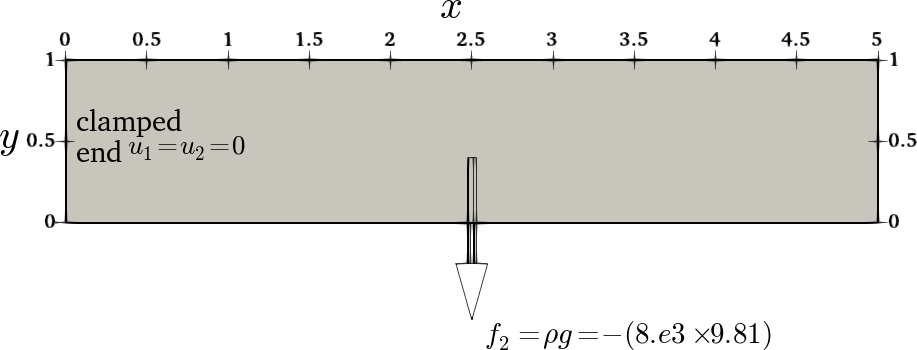
\includegraphics[align=t,width=.44\textwidth]{2d-bar.png}\hspace{.1\textwidth}
    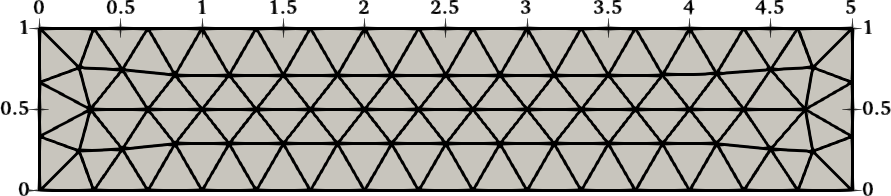
\includegraphics[align=t,width=.44\textwidth]{2d-bar-mesh.png}
    \caption{2D bar clamped at left end and bending under own load. Geometry (left) and mesh (right).}
    \label{fig:2Dbar}
\end{figure} 

\textbf{Step 1: Preprocessing}

First step in a PSD simulation is ``PSD setup", at this step you tell PSD what kind of physics, boundary conditions, approximations, mesh, etc are you expecting to solve.
For ``PSD setup" go to the {\ttfamily PSD/Solver} folder, launch the terminal there and run the following command.
\begin{lstlisting}[style=Linux]
PSD_PreProcess -dimension 2 -bodyforce  -dirichletconditions 1 -plot
\end{lstlisting}
%
After the ``PSD setup" runs successfully you should see many {\ttfamily .edp} files in your {\ttfamily PSD/Solver} folder. \textit{What do the arguments mean ?} {\ttfamily SolverGenerator.edp} is the file that is responsible for creating additional files in your {\ttfamily PSD/Solver} folder; {\ttfamily -dimension 2} means it is a 2D simulation, {\ttfamily -bodyforce} with body force; {\ttfamily -dirichletconditions 1} says we have one Dirichlet border; and {\ttfamily -plot} means we would like to have ParaView post processing files. The input properties ``$E,\nu, \mathbf{f}$" can be changed in {\ttfamily ControlParameters.edp} by changing {\ttfamily E, nu, f$_2$}. These are changed to {\ttfamily E  = 200.e9}, {\ttfamily nu = 0.3;}, {\ttfamily f$_2$=8.e3*(-9.81);}. Note, {\ttfamily f$_2$} is the second component of $\mathbf{f}$. Dirichlet boundary conditions are also provided in {\ttfamily ControlParameters.edp}. To provide Dirichlet label (clamped end), the vector {\ttfamily int[int] Dlabel = [2];} should be used, here we assume that the label number of the left end is 2. For this clamped end $u_1=u_2=0$, this is provided by {\ttfamily real[int]   Dvalue = [0.,0.];}.

\textbf{Step 2: Solving}

As PSD is a parallel solver, let us use  4 cores to solve the 2D bar case. To do so enter the following command:

\begin{lstlisting}[style=Linux]
ff-mpirun -np 4 Main.edp
\end{lstlisting}

Here {\ttfamily -np 4} denote the argument used to enter the number of cores. Note that if your problem is large use more cores. PSD has been tested upto 13,000 cores, surely you will now need that many for the 2D bar problem. 

\textbf{Step 3: Postprocessing}

PSD allows postprocessing of results in ParaView. After the step 2 mentioned above finishes. Launch ParaView and have a look at the  {\ttfamily .pvd} file in the  {\ttfamily PSD/Solver/VTUs\_DATE\_TIME} folder. 

\begin{figure}[htbp]
    \centering
    \begin{minipage}[t][2cm][t]{0.4\textwidth}
    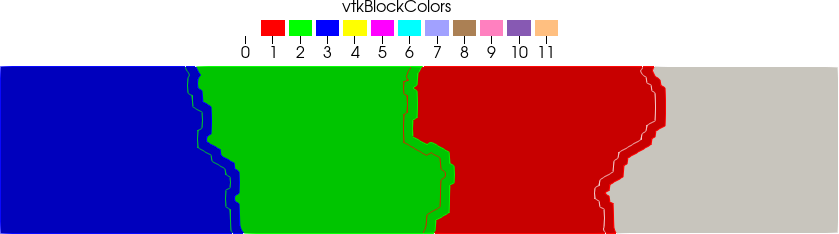
\includegraphics[align=t,width=1\textwidth]{2d-bar-partioned.png}
    \end{minipage}\hspace{.1\textwidth}
    \begin{minipage}[t][2cm][t]{0.4\textwidth}
    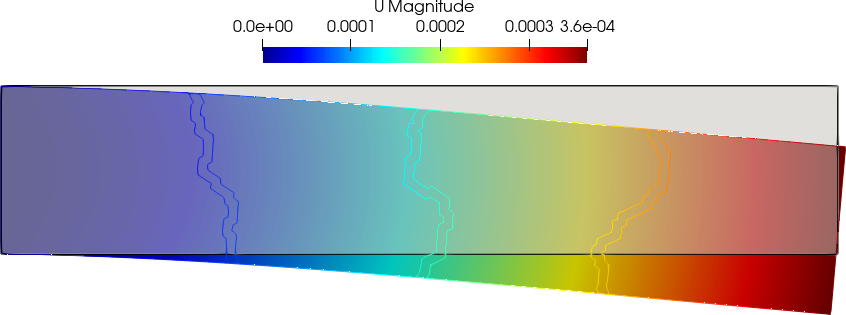
\includegraphics[align=t,width=1\textwidth]{2d-bar-results.png}
    \end{minipage}
    \caption{2D clamped bar results. Partitioned mesh (left) and 1000X warped displacement field (right).}
    \label{fig:2d-bar-results}
\end{figure}


\subsection{PSD simulation of 2D bar problem clamped at both ends \label{sec:2D-bar-clamped1}}

For this test the properties of the material are the same as used in \cref{sec:2d-bar-load}. 

\textbf{Step 1: Preprocessing}

For ``PSD setup" go to the {\ttfamily PSD/Solver} folder, launch the terminal there and run the following command.
\begin{lstlisting}[style=Linux]
PSD_PreProcess -dimension 2 -plot -dirichletconditions 2 -bodyforce
\end{lstlisting}
%
Since basic nature of both the problems is same this is the exact same command used in preprocessing of \cref{sec:2d-bar-load}. The only difference of this problem compared to the one from \cref{sec:2d-bar-load} is that an additional Dirichlet condition needs to be supplied, notified to PSD by {\ttfamily -dirichletconditions 2}. To provide Dirichlet label of the two clamped end in {\ttfamily ControlParameters.edp} the vector {\ttfamily int[int] Dlabel = [2,4];} should be used, here we assume that the label number of the left end is 2 and right end is 4. For these clamped end $u_1=u_2=0$, this is provided by {\ttfamily real[int]   Dvalue = [0.,0.,0.,0.];}. In the  {\ttfamily real[int]   Dvalue = [0.,0.,0.,0.];} the fist two digits correspond to $u_1,u_2$ of label 2 and the last two digits correspond to $u_1,u_2$ of label 4.



\textbf{Step 2: Solving}

Let us now use  3 cores to solve this problem. To do so enter the following command:

\begin{lstlisting}[style=Linux]
ff-mpirun -np 3 Main.edp
\end{lstlisting}
%
Notice, that this is the exact same command used in solving of \cref{sec:2d-bar-load}, with only difference that we now use {\ttfamily -np 3} vs.~{\ttfamily -np 4}.


\textbf{Step 3: Postprocessing}

Launch ParaView and have a look at the  {\ttfamily .pvd} file in the  {\ttfamily PSD/Solver/VTUs\_DATE\_TIME} folder. 

\begin{figure}[htbp]
    \centering
    \begin{minipage}[t][2cm][t]{0.4\textwidth}
    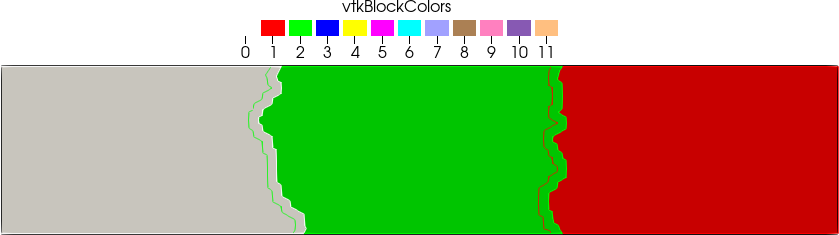
\includegraphics[align=t,width=1\textwidth]{2d-bar-partitioned3.png}
    \end{minipage}\hspace{.1\textwidth}
    \begin{minipage}[t][2cm][t]{0.4\textwidth}
    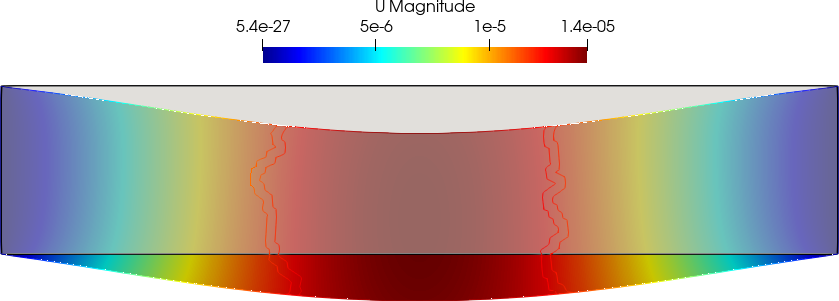
\includegraphics[align=t,width=1\textwidth]{2d-bar-clamped-ends.png}
    \end{minipage}
    \caption{2D clamped bar results. Partitioned mesh (left) and 20000X warped displacement field (right).}
    \label{fig:3part}
\end{figure}

In~\cref{fig:3part} there are only three subdomais in the partitioned mesh since only three cores were used.

\subsubsection{Redoing the test on Jupiter and moon}

Imagine, you wish to know how the test would compare if performed on Moon and Jupiter. The only thing that will change now is the gravitational pull, for Moon $g=1.32$ and for Jupiter $g=24.79$. To perform the moon test simply change  {\ttfamily f$_2$=8.e3*(-1.32);} in {\ttfamily ControlParameters.edp} and redo step 2 and step 3. Similarly for the Jupiter test {\ttfamily f$_2$=8.e3*(-24.79);} in {\ttfamily ControlParameters.edp} and redo step 2 and step 3.

\begin{figure}[htbp]
    \centering
    \begin{minipage}[t][2.5cm][t]{0.4\textwidth}
    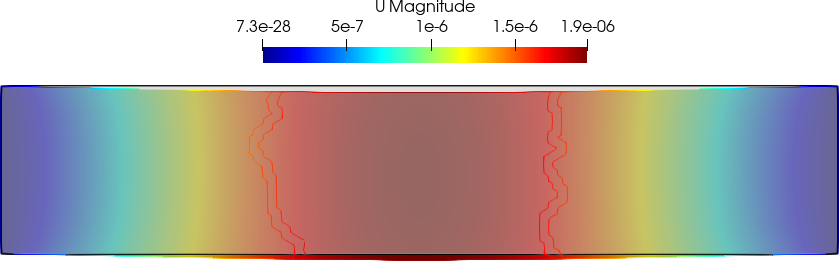
\includegraphics[align=t,width=1\textwidth]{2d-bar-moon.png}
    \end{minipage}\hspace{.1\textwidth}
    \begin{minipage}[t][2.5cm][t]{0.4\textwidth}
    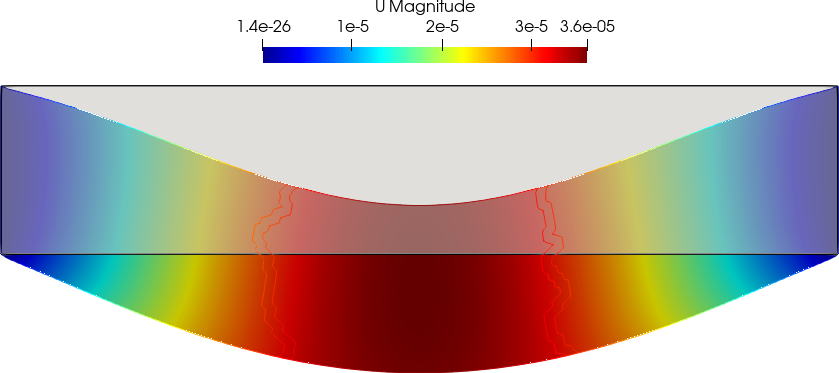
\includegraphics[align=t,width=1\textwidth]{2d-bar-Jupiter.png}
    \end{minipage}
    \caption{2D clamped bar 20000X warped displacement fields. On moon (left) and  on Jupiter (right).}
    \label{fig:moon-jupiter}
\end{figure}

\subsection{PSD simulation of 2D bar problem clamped at one end wile being pulled at the other end (Dirichlet-Dirichlet case)\label{sec:2d-bar-clamped2}}

In this section we showcase the 2D bar problem simulation with one end clamped wile being pulled at the other end. Body force is neglected and the non clamped ends pull is approximated with Dirichlet displacement $u_1=1$. If this simulation is compared to the previous one from \cref{sec:2d-bar-load}, the only difference now is that no body force is applied and an additional Dirichlet condition is applied at the free end of the bar. Here is how PSD simulation of this case can be performed.

\textbf{Step 1: Preprocessing}

For ``PSD setup" go to the {\ttfamily PSD/Solver} folder, launch the terminal there and run the following command.
\begin{lstlisting}[style=Linux]
PSD_PreProcess -dimension 2 -dirichletconditions 2 -plot
\end{lstlisting}
%
In comparison to preprocessing from \cref{sec:2d-bar-load,sec:2D-bar-clamped1}, notice that {\ttfamily -bodyforce} is missing. This is due to the fact that for this problem we assume zero body force. Just like in~\cref{sec:2D-bar-clamped1} {\ttfamily -dirichletconditions 2}, which notifies to PSD that there are two Dirichlet borders ---the clamped and the pulled ends of the bar--- in this simulation. To add the values and label numbers of the Dirichlet borders edit the  {\ttfamily ControlParameters.edp},  the vector {\ttfamily int[int] Dlabel = [2,4];} should be used, here we assume that the label number of the left end is 2 and right end is 4. For the left end $u_1=0,u_2=0$ and for the right end $u_1=1,u_2=0$, this is provided by {\ttfamily real[int]   Dvalue = [0.,0.,1.,0.];}. In the  {\ttfamily real[int]   Dvalue = [0.,0.,0.,0.];} the fist two digits correspond to $u_1,u_2$ of label 2 and the last two digits correspond to $u_1,u_2$ of label 4. Note that here at border 4 we have explicitly set $u_2=0$ this means the bar is not allowed to shrink in $y$ direction (compress), however you might wish to allow the bar to compress. Such a simulation requires a little bit of more editing in preprocessing step, we shall deal with this in the later tutorials, for now we focus on the current case. So now PSD should be ready to solve. 

\textbf{Step 2: Solving}

Let us now use 2 cores to solve this problem. To do so enter the following command:

\begin{lstlisting}[style=Linux]
ff-mpirun -np 2 Main.edp
\end{lstlisting}
%
Notice, that this is the exact same command used in solving of \cref{sec:2d-bar-load,sec:2D-bar-clamped1}, with only difference that we now use {\ttfamily -np 2} vs.~{\ttfamily -np 4} in \cref{sec:2d-bar-load} and ~{\ttfamily -np 3} in \cref{sec:2D-bar-clamped1}.


\textbf{Step 3: Postprocessing}

Launch ParaView and have a look at the  {\ttfamily .pvd} file in the  {\ttfamily PSD/Solver/VTUs\_DATE\_TIME} folder. 

\begin{figure}[htbp]
    \centering
    \begin{minipage}[t][2cm][t]{0.39\textwidth}
    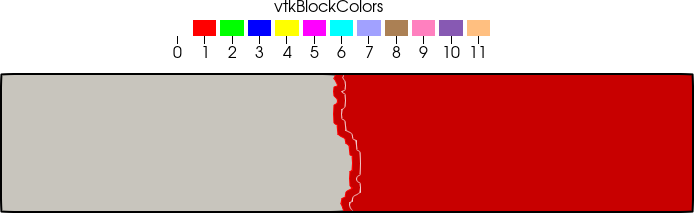
\includegraphics[align=t,width=1\textwidth]{2d-bar-clamped-pulled-partioned.png}
    \end{minipage}\hspace{.1\textwidth}
    \begin{minipage}[t][2cm][t]{0.5\textwidth}
    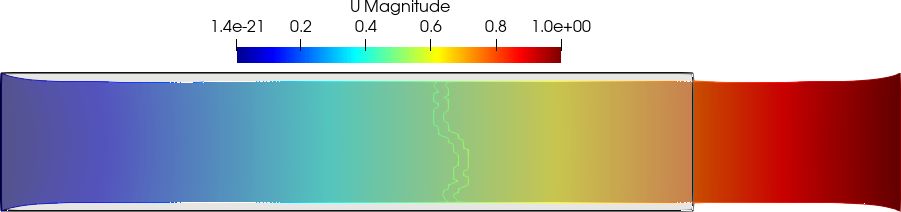
\includegraphics[align=t,width=1\textwidth]{2d-bar-clamped-pulled.png}
    \end{minipage}
    \caption{2D bar results. Partitioned mesh (left) and 1.5X warped displacement field (right).}
    \label{fig:2part}
\end{figure}

Note now in~\cref{fig:2part} there are only two subdomais in the partitioned mesh since only three cores were used. As expected we see that the right end of the bar which is being pulled does not contract in $y$ direction.
\pagebreak


\subsection{PSD simulation of 2D bar problem clamped at one end wile being pulled at the other end (Dirichlet--Neumann case)\label{sec:2d-bar-clamped3}}


Similar simulation, as in \cref{sec:2d-bar-clamped2} is presented in this section. We showcase the 2D bar problem simulation with one end clamped wile being pulled at the other end. Just like simulation from \cref{sec:2d-bar-clamped2} the body force is neglected, However now  the non clamped ends pull is approximated with Neumann force $\int_{\partial\Omega^h_{\text N}}(\mathbf t\cdot \bvh)$. To simulate the pull we assume traction vector $\mathbf t=[t_1,t_2]=[10^9.,0]$ acting on the non clamped right end of the bar, i.e., force in $x$ direction is 10 units. Here is how PSD simulation of this case can be performed.

\textbf{Step 1: Preprocessing}

For ``PSD setup" go to the {\ttfamily PSD/Solver} folder, launch the terminal there and run the following command.
\begin{lstlisting}[style=Linux]
PSD_PreProcess -dimension 2 -dirichletconditions 1  -tractionconditions 1 -plot
\end{lstlisting}
%
the comandline flag {\ttfamily -dirichletconditions 1}, notifies to PSD that there is one Dirichlet border ---the clamped end of the bar--- in this simulation. And the flag {\ttfamily -tractionconditions 1} notifies to PSD that there is one traction border ---the right end of the bar--- in this simulation. 
To add the values and label numbers of the Dirichlet borders edit the  {\ttfamily ControlParameters.edp},  the vector {\ttfamily int[int] Dlabel = [2];} should be used, here we assume that the label number of the left end is 2. For the left end $u_1=0,u_2=0$ hence in {\ttfamily ControlParameters.edp}, use {\ttfamily real[int]   Dvalue = [0.,0.];}. To add the values and label numbers of the traction borders edit the  {\ttfamily ControlParameters.edp},  the vector {\ttfamily int[int] Tlabel = [4];} should be used, here we assume that the label number of the right end is 4. For this end $\mathbf t=[t_1,t_2]=[10^9.,0]$, hence in {\ttfamily ControlParameters.edp}, use {\ttfamily real  tx0=1.e9, ty0=0.;}. 


\textbf{Step 2: Solving}

Let us now use 5 cores to solve this problem. To do so enter the following command:

\begin{lstlisting}[style=Linux]
ff-mpirun -np 5 Main.edp
\end{lstlisting}
%
Notice, that this is the exact same command used in solving the previous bar problems from other sections, with only difference that we now use {\ttfamily -np 5}.


\textbf{Step 3: Postprocessing}

Launch ParaView and have a look at the  {\ttfamily .pvd} file in the  {\ttfamily PSD/Solver/VTUs\_DATE\_TIME} folder. 

\begin{figure}[htbp]
    \centering
    \begin{minipage}[t][2cm][t]{0.36\textwidth}
    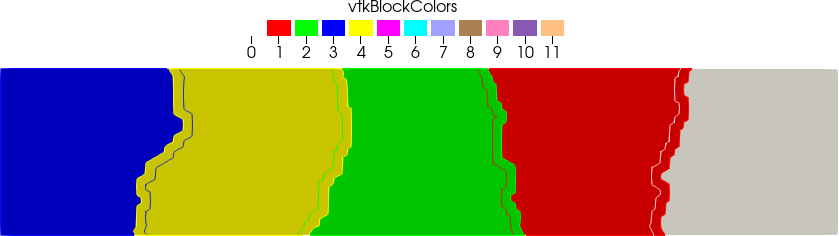
\includegraphics[align=b,width=1\textwidth]{2d-bar-partitioned5.png}
    \end{minipage}\hspace{.1\textwidth}
    \begin{minipage}[t][2cm][t]{0.5\textwidth}
    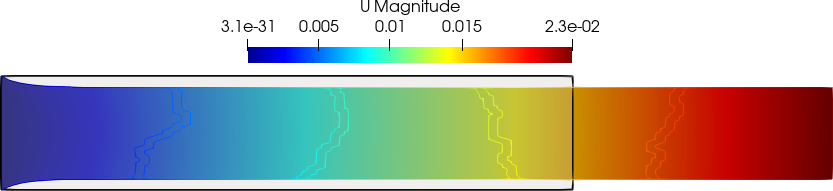
\includegraphics[align=b,width=1\textwidth]{2d-bar-clamped-traction.png}
    \end{minipage}
    \caption{2D bar results. Partitioned mesh (left) and 100X warped displacement field (right).}
    \label{fig:5part}
\end{figure}

Note now in~\cref{fig:5part} there are five subdomais in the partitioned mesh since five cores were used. Contrary to~\cref{fig:2part}, as expected, we see that the right end of the bar which is being pulled now contract in $y$ direction. This is due to the fact that there is no Dirichlet condition at this end now. 

\pagebreak




\subsection{PSD simulation of 2D bar problem clamped at one end wile being pulled at the other end (Dirichlet-Neumann-Point boundary conditions case)\label{sec:2d-bar-clamped4}}


Similar simulations, as in \cref{sec:2d-bar-clamped2,sec:2d-bar-clamped3} is presented in this section. We showcase the 2D bar problem simulation with one end clamped  wile being pulled at the other end. Contrary to simulation in \cref{sec:2d-bar-clamped2,sec:2d-bar-clamped3}, the clamped end just restricts $x$ movement, i.e, $u_1=0$. Just like simulation from \cref{sec:2d-bar-clamped2,sec:2d-bar-clamped3} the body force is neglected. Just like simulation in  \cref{sec:2d-bar-clamped3}, the non clamped ends pull is approximated with Neumann force $\int_{\partial\Omega^h_{\text N}}(\mathbf t\cdot \bvh)$. To simulate the pull we assume traction vector $\mathbf t=[t_1,t_2]=[10^9,0]$ acting on the non clamped right end of the bar, i.e., force in $x$ direction is $10^9$ units. Here is how PSD simulation of this case can be performed.


\textbf{Step 1: Preprocessing}

For ``PSD setup" go to the {\ttfamily PSD/Solver} folder, launch the terminal there and run the following command.
\begin{lstlisting}[style=Linux]
PSD_PreProcess -dimension 2 -dirichletconditions 1 -tractionconditions 1 -dirichletpointconditions 1 -plot
\end{lstlisting}

Additional flag {\ttfamily -dirichletpointconditions 1} now appears, this notifies to PSD that there is one Dirichlet point boundary condition. To add the values and label numbers of the Dirichlet borders which contains this point edit the  {\ttfamily ControlParameters.edp},  the vector {\ttfamily int[int] Dpointlab = [2];} should be used, here we assume that the label number of the left end is 2 and that left end contains our Dirichlet point. For this point $x=y=0$ and $u_1=0,u_2=0$ to specify this in {\ttfamily ControlParameters.edp}, use {\ttfamily PnV = [ 0., 0., 0., 0.];} which is infact a vector of $[x,y,u_1,u_2]$. Via the flags we specified that {\ttfamily -dirichletconditions 1}, i.e., there is one Dirichlet border. However now in this simulation the border only has one Dirichlet condition $u_1=0$, while $u_2$ is free. This condition needs editing of {\ttfamily VariationalFormulations.edp}, comment or remove the line {\ttfamily u1 = Dvalue[1]}. Commenting or removing this line lets free {\ttfamily u1} which is infact $u_2$. Note that this is due to the fact that in PSD $[u_1,u_2,u_3]$ maps to {\ttfamily [u,u1,u2]}.

\textbf{Step 2: Solving}

Let us now use 6 cores to solve this problem. To do so enter the following command:

\begin{lstlisting}[style=Linux]
ff-mpirun -np 5 Main.edp
\end{lstlisting}
%
Notice, that this is the exact same command used in solving the previous bar problems from other sections, with only difference that we now use {\ttfamily -np 6}.


\textbf{Step 3: Postprocessing}

Launch ParaView and have a look at the  {\ttfamily .pvd} file in the  {\ttfamily PSD/Solver/VTUs\_DATE\_TIME} folder. 

\begin{figure}[htbp]
    \centering
    \begin{minipage}[t][2cm][t]{0.36\textwidth}
    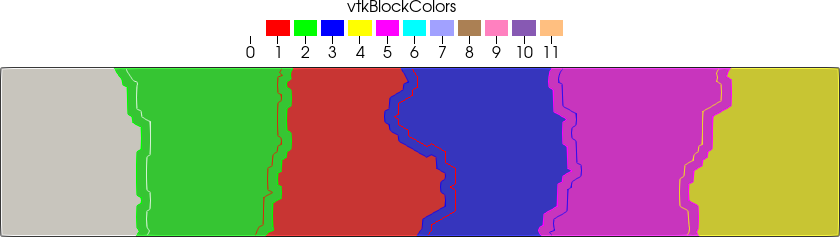
\includegraphics[align=b,width=1\textwidth]{2d-bar-partitioned6.png}
    \end{minipage}\hspace{.1\textwidth}
    \begin{minipage}[t][2cm][t]{0.5\textwidth}
    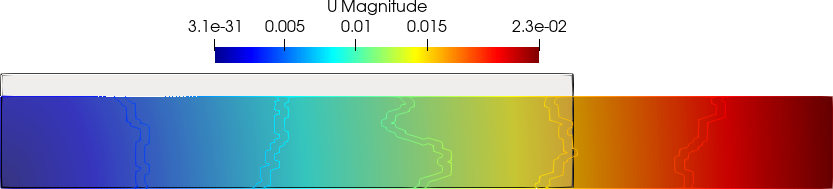
\includegraphics[align=b,width=1\textwidth]{2d-bar-clamped-traction-point.png}
    \end{minipage}
    \caption{2D bar results. Partitioned mesh (left) and 100X warped displacement field (right).}
    \label{fig:6part}
\end{figure}

Note now in~\cref{fig:6part} there are six subdomais in the partitioned mesh. As expected, we see that the right and the left end of the bar which is being pulled now contract in $y$ direction, and the bar elongates in $x$ direction. 


\pagebreak



\subsection{PSD simulation of 3D bar problem clamped at one end wile being pulled at the other end (Dirichlet-Neumann case)\label{sec:3d-bar-clamped3}}

In this section we present a 3D PSD simulation of a clamped bar which his being loaded in vertical direction at the non-clamped end. This simulation is like the one presented in \cref{sec:2d-bar-clamped3}, however in 3D. The material properties are same as before, and at the non-clamped end traction $t_y=-10^9$ units. The 3D bar is $1\times1\times5$ m$^3$.

Here is how PSD simulation of this case can be performed.

\textbf{Step 1: Preprocessing}

For ``PSD setup" go to the {\ttfamily PSD/Solver} folder, launch the terminal there and run the following command.
\begin{lstlisting}[style=Linux]
PSD_PreProcess -dimension 3 -dirichletconditions 1  -tractionconditions 1 -plot
\end{lstlisting}
%
the comandline flag {\ttfamily -dirichletconditions 1} notifies to PSD that there is one Dirichlet border ---the clamped end of the bar--- in this simulation; {\ttfamily -dimension 3} means the simulation is 3D. And the flag {\ttfamily -tractionconditions 1} notifies to PSD that there is one traction border ---the right end of the bar--- in this simulation. 
To add the values and label numbers of the Dirichlet borders edit the  {\ttfamily ControlParameters.edp},  the vector {\ttfamily int[int] Dlabel = [1];} should be used, here we know that the label number of the left clamped end is 1. For the left end $u_1=0,u_2=0,u_3=0$ hence in {\ttfamily ControlParameters.edp}, use {\ttfamily real[int]   Dvalue = [0.,0.,0.];}. To add the values and label numbers of the traction borders edit the  {\ttfamily ControlParameters.edp},  the vector {\ttfamily int[int] Tlabel = [2];} should be used, here we know that the label number of the right end is 2. For this end $\mathbf t=[t_1,t_2,t_3]=[0.,10^9,0.]$, hence in {\ttfamily ControlParameters.edp}, use {\ttfamily real  tx0=0., ty0=1.e9, tz0=0.,;}. 


\textbf{Step 2: Solving}

Let us now use 4 cores to solve this problem. To do so enter the following command:

\begin{lstlisting}[style=Linux]
ff-mpirun -np 4 Main.edp
\end{lstlisting}
%
Notice, that this is the exact same command used in solving the previous bar problems from other sections.


\textbf{Step 3: Postprocessing}

Launch ParaView and have a look at the  {\ttfamily .pvd} file in the  {\ttfamily PSD/Solver/VTUs\_DATE\_TIME} folder. 

\begin{figure}[htbp]
    \centering
    \begin{minipage}[t][2cm][t]{0.38\textwidth}
    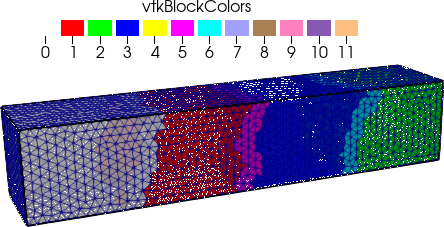
\includegraphics[align=b,width=1\textwidth]{3d-bar-clamped-ends.png}
    \end{minipage}\hspace{.1\textwidth}
    \begin{minipage}[t][2cm][t]{0.4\textwidth}
    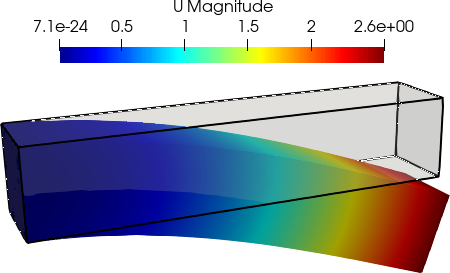
\includegraphics[align=b,width=1\textwidth]{3d-bar-clamped-pulled-partioned.png}
    \end{minipage}
    \caption{3D bar results. Partitioned mesh (left) and 0.5X warped displacement field (right).}
    \label{fig:3Dpart}
\end{figure}

In~\cref{fig:3Dpart} there are four subdomais in the partitioned mesh since four cores were used.

\pagebreak


\subsection{PSD simulation of 3D  mechanical piece (Dirichlet-Neumann case) with complex mesh\label{sec:3d-bar-clamped3-sub}}

So far in the previous cases we only concentrated on bar simulations, which were more or less trivial cases. Moreover, the bar meshes are provided with the PSD solver. In this section we now turn towards  3D simulation of a mechanical piece, the geometry of which is shown in~\cref{fig:mechanicalpiecegeo}. The left (small) hole is fixed: $u_1=u_2=u_3=0$, while as traction force $t_x=10^9$ is applied on the large hole.

You can grab a copy of CAD geometry for the mechanical piece (the Gmsh {\ttfamily .geo}) your local Gmsh installation folder  {\ttfamily gmsh/share/doc/gmsh/demos/simple\_geo/{piece}.geo}. The listing of the file is also given in @. To generate the mesh {\ttfamily piece.msh} simply do 
\begin{lstlisting}[style=Linux]
gmsh -3 piece.geo
\end{lstlisting}
Place the generated mesh {\ttfamily piece.msh} in {\ttfamily /PSD/Meshes/3D/piece.msh}. Now the PSD simulation can be performed.

\begin{figure}[h]
    \centering
    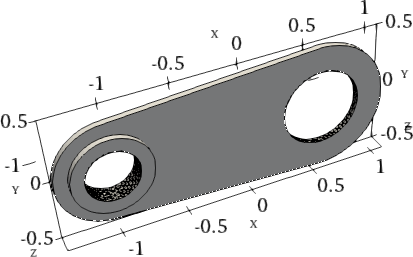
\includegraphics[align=b,width=0.5\textwidth]{3d-mechanical.png}
    \caption{3D mechanical piece.}
    \label{fig:mechanicalpiecegeo}
\end{figure}

\textbf{Step 1: Preprocessing}

For ``PSD setup" go to the {\ttfamily PSD/Solver} folder, launch the terminal there and run the following command.
\begin{lstlisting}[style=Linux]
PSD_PreProcess -dimension 3 -dirichletconditions 1  -tractionconditions 1 -plot
\end{lstlisting}
Here, by using these parameters we have generated one Dirichlet condition and one traction condition, respectively to be applied to the small and the large holes in the mesh. Further, by using {\ttfamily -dimension 3} we have let PSD know that the problem is 3D .In the {\ttfamily /PSD/Meshes/3D/piece.msh} generated, the label 4 (resp.~3) corresponds to the Dirichlet (resp.~traction) border. To add the values and label numbers of the Dirichlet borders edit the  {\ttfamily ControlParameters.edp},  the vector {\ttfamily int[int] Dlabel = [4];} should be used. For this label $u_1=0,u_2=0,u_3=0$ hence in {\ttfamily ControlParameters.edp}, use {\ttfamily real[int]   Dvalue = [0.,0.,0.];}. To add the values and label numbers of the traction borders edit the  {\ttfamily ControlParameters.edp},  the vector {\ttfamily int[int] Tlabel = [3];} should be used. For this end $\mathbf t=[t_1,t_2,t_3]=[0.,10^9,0.]$, hence in {\ttfamily ControlParameters.edp}, use {\ttfamily real  tx0=0., ty0=1.e9, tz0=0.,;}. Finally we use steel properties for the material, so in {\ttfamily ControlParameters.edp} the parameters {\ttfamily real E  = 200.e9;} and {\ttfamily real nu = 0.3;} should be used. These represent $E$ and $\nu$, respectively. With all the properties and boundary conditions set we now use  {\ttfamily string ThName = "../Meshes/3D/piece";} in the {\ttfamily ControlParameters.edp} file, this notifies PSD about the name of the mesh used for this simulation.  

\textbf{Step 2: Solving}

Let us now use 2 cores to solve this problem. To do so enter the following command:

\begin{lstlisting}[style=Linux]
ff-mpirun -np 2 Main.edp
\end{lstlisting}

\textbf{Step 3: Postprocessing}

Launch ParaView and have a look at the  {\ttfamily .pvd} file in the  {\ttfamily PSD/Solver/VTUs\_DATE\_TIME} folder. 

\begin{figure}[htbp]
    \centering
    \begin{minipage}[t][2cm][t]{0.36\textwidth}
    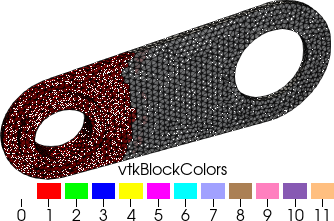
\includegraphics[align=b,width=1\textwidth]{3d-mechanical-part.png}
    \end{minipage}\hspace{.1\textwidth}
    \begin{minipage}[t][2cm][t]{0.4\textwidth}
    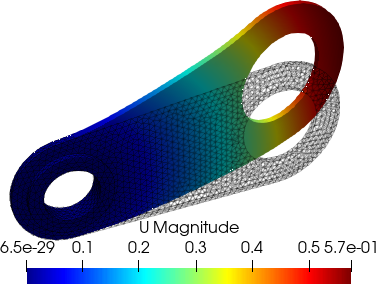
\includegraphics[align=b,width=1\textwidth]{3d-mechanical-result.png}
    \end{minipage}
    \caption{Mechanical piece test results. Partitioned mesh (left) and  warped displacement field (right).}
    \label{fig:mechapieceresult}
\end{figure}

\textbf{Redoing the test with different conditions}

\begin{figure}[htbp]
    \centering
    \begin{minipage}{0.42\textwidth}
    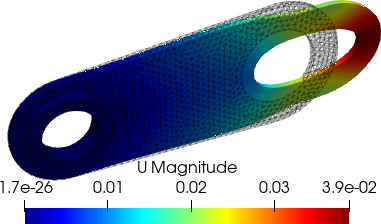
\includegraphics[align=b,width=1\textwidth]{3d-mechanical-result-x.png}
    \subcaption{{\ttfamily real  tx0=1.e9, ty0=0, tz0=0.,;}}
    \end{minipage}\hspace{.1\textwidth}
    \begin{minipage}{0.4\textwidth}
    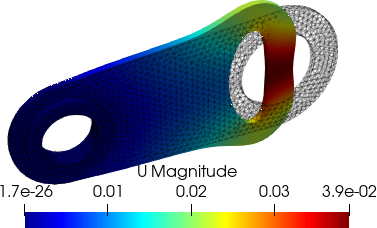
\includegraphics[align=b,width=1\textwidth]{3d-mechanical-result--x.png}
    \subcaption{{\ttfamily real  tx0=1.e9, ty0=0, tz0=0.,;}}
    \end{minipage}
    \caption{Mechanical piece test results.}
    \label{fig:mechapieceresult2}
\end{figure}



\pagebreak













\section{Damage mechanics}
\subsection{Hybrid phase-field for damage}
On a meshed domain $\Omega^h\in\Omega\subset\mathbb{R}^n$, for damage mechanics the mixed finite element variational formulation in the Lagrangian framework for searching the unknown nodal displacements vector $\bu^h=[u_1,u_2,u_3]^\mathsf{T}$ reads,
%
%
\begin{equation}\label{Eq:VarfU}
\begin{aligned}
&\text{search}~\buh\in\mathbb{V}^h \text{~that satisfies}~\forall\, t\in[0,T]:\\
&\int_{\Omega^h}\big[(1-d^h)^2 + \kappa \big]\sig(\buh) : \eps(\bvh) \,\dv= \int_{\partial\Omega^h_\text{N}} \overline{\bt}\cdot\bvh \,\ds \quad\forall\,\bv^h\in\mathbb{V}^h,
\end{aligned}
\end{equation}
where $\kappa\ll1$ is a model parameter to prevent numerical singularity when $d \to 1$.
 %
 %
In this formulation, the notation ``$:$" is used for the double contraction between tensors (i.e., component-wise tensor product) and $ \mathbb{V}^h $ is a  mixed third order vector valued finite element functional space to approximate vector test function~$\bvh$ and vector trial function~$\buh$:
 %
\begin{equation}
\mathbb{V}^h=\left\{ \bu^h\in [ {H}^1(\Omega^h) ]^3~~\forall t\in[0,T]~|~ \forall \bx\in\partial\Omega^h_{\text{D}}~\buh=\overline{\bu}\right\},
\end{equation}
%
with ${H}^1(\Omega^h)$ denoting a square integrable Sobolev functional space.
Similarly, for~the phase-field the standard finite element variational formulation for the unknown damage scalar $\fih$ reads, 
%
%
\begin{equation}
\begin{aligned}\label{Eq:VarfPhi}
&\text{search}~\fih\in{{V}}^h \text{~that satisfies}~\forall\, t\in[0,T]:\\
&\int_{\Omega^h}\left[ \frac{\bgc}{l_0} + 2 \mathcal{H}^{+}(\buh) \right]\fih\ttah\, \dv + \int_{\Omega^h} {\bgc}{l_0}\nabla\fih \cdot \nabla\ttah \, \dv= \int_{\Omega^h} 2\mathcal{H}^{+}(\buh)\ttah \, \dv\quad\forall\,\ttah\in{{V}}^h, 
\end{aligned}
\end{equation}
%
%
where,~${{V}}^h$ denotes the scalar finite element functional space to approximate scalar test function~$\ttah$ and scalar trial function~$\fih$:
\begin{equation}
{{V}}^h=\left\{\fih \in  {H}^1(\Omega^h)~~\forall t\in[0,T]~\middle|~\fih\in[0,1]  \right\}.
\end{equation}

\pagebreak

\section{Elastodynamics}
\pagebreak

\section{Soil dynamics}



\pagebreak

\lstset{
  language={PSD},
  basicstyle=\small\ttfamily, % Global Code Style
  captionpos=b, % Position of the Caption (t for top, b for bottom)
  extendedchars=true, % Allows 256 instead of 128 ASCII characters
  tabsize=2, % number of spaces indented when discovering a tab 
  columns=fixed, % make all characters equal width
  keepspaces=true, % does not ignore spaces to fit width, convert tabs to spaces
  showstringspaces=false, % lets spaces in strings appear as real spaces
  breaklines=true, % wrap lines if they don't fit
  frame=trbl, % draw a frame at the top, right, left and bottom of the listing
  frameround=tttt, % make the frame round at all four corners
  framesep=4pt, % quarter circle size of the round corners
  numbers=left, % show line numbers at the left
  numberstyle=\tiny\ttfamily, % style of the line numbers
  commentstyle=\color{eclipseGreen}, % style of comments
  keywordstyle=\color{eclipsePurple}, % style of keywords
  stringstyle=\color{eclipseBlue}, % style of strings
}



\begin{lstlisting}[language=PSD]
import math
import numpy as np
from lib.analytical import csa

sin2_theta  = np.sin(theta)**2  // THis is  a commen
+= -= *= /= + - * / ? < > & % == <=
# += -= *= /= + - * / ? < > & % == <=
def test(a=100, b=True):
    <= >= == 2 + 3j * 7e-3
\end{lstlisting}

\chapter{Validation}


\chapter{Functions and descriptions}
\section{Flag descriptions}
\begin{description}

\item[-dimension] Takes in datatype {\ttfamily int}. With this flag the dimension of the problem can be set, for a 2D problem {\ttfamily -dimension 2}, and for a 3D problem {\ttfamily -dimension 3}. Default is 2.

\item[-help] This is a boolean flag. With this flag some  helping messages are printed on the terminal. 

\item[-plot] This is a boolean flag. To activate postprocessing via ParaView. 

\item[-useGFP] This is a boolean flag. To activate GoFastPlugins support for PSD (A suite of c++ plugins). 

\item[-useRCM] This is a boolean flag. To activate mesh level renumbering via Reverse Cuthill Mckee. 

\item[-dynamic] This is a boolean flag. To generate a dynamic solver. 



\end{description}

\chapter{Gallery}

This chapter showcases some test cases that have been performed with PSD.

\begin{figure}
    \centering
    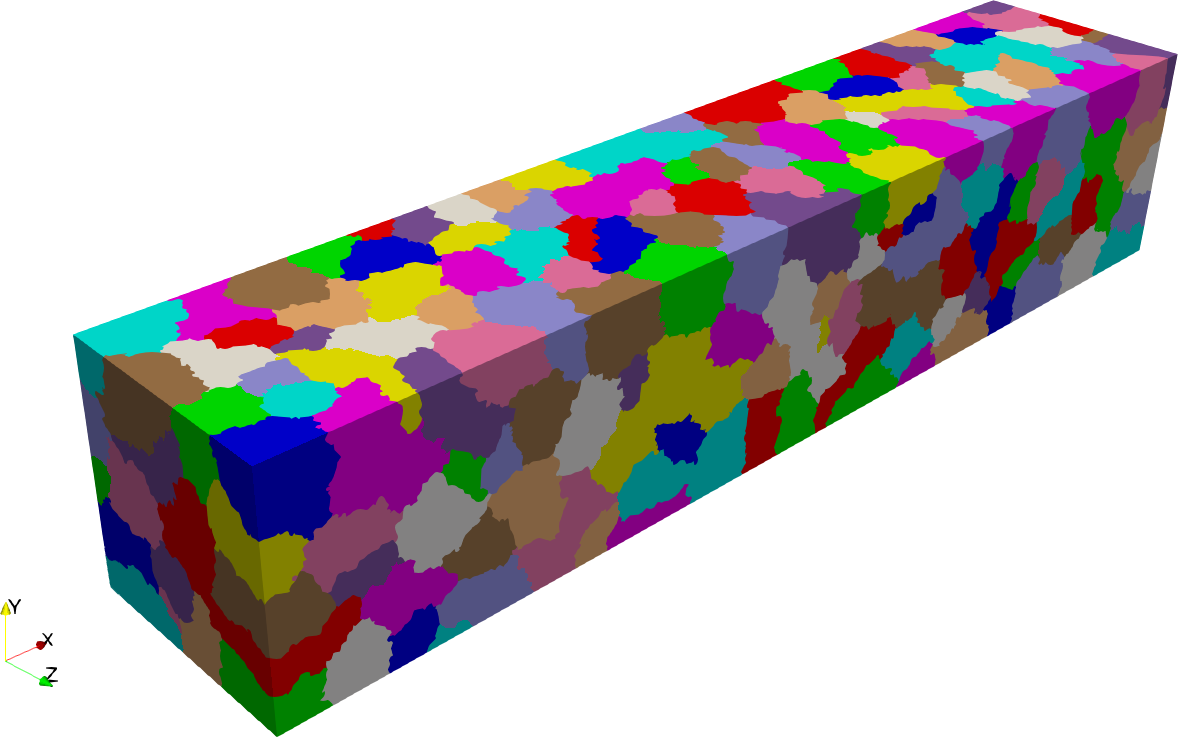
\includegraphics[width=0.5\textwidth]{400partmesh3d.png}
    \caption{90 M dof with 400 partitions.}
    \label{fig:90Mdof}
\end{figure}

\begin{figure}
    \centering
    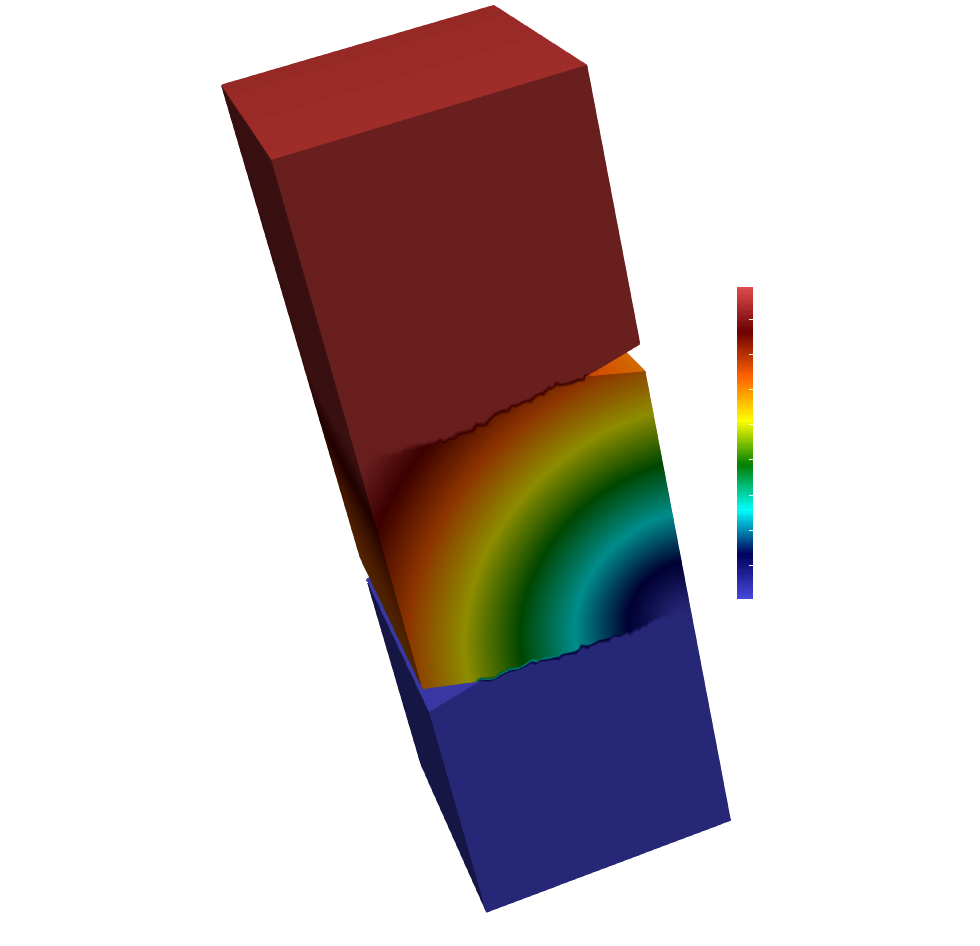
\includegraphics[width=0.45\textwidth]{rainbow-test.png}    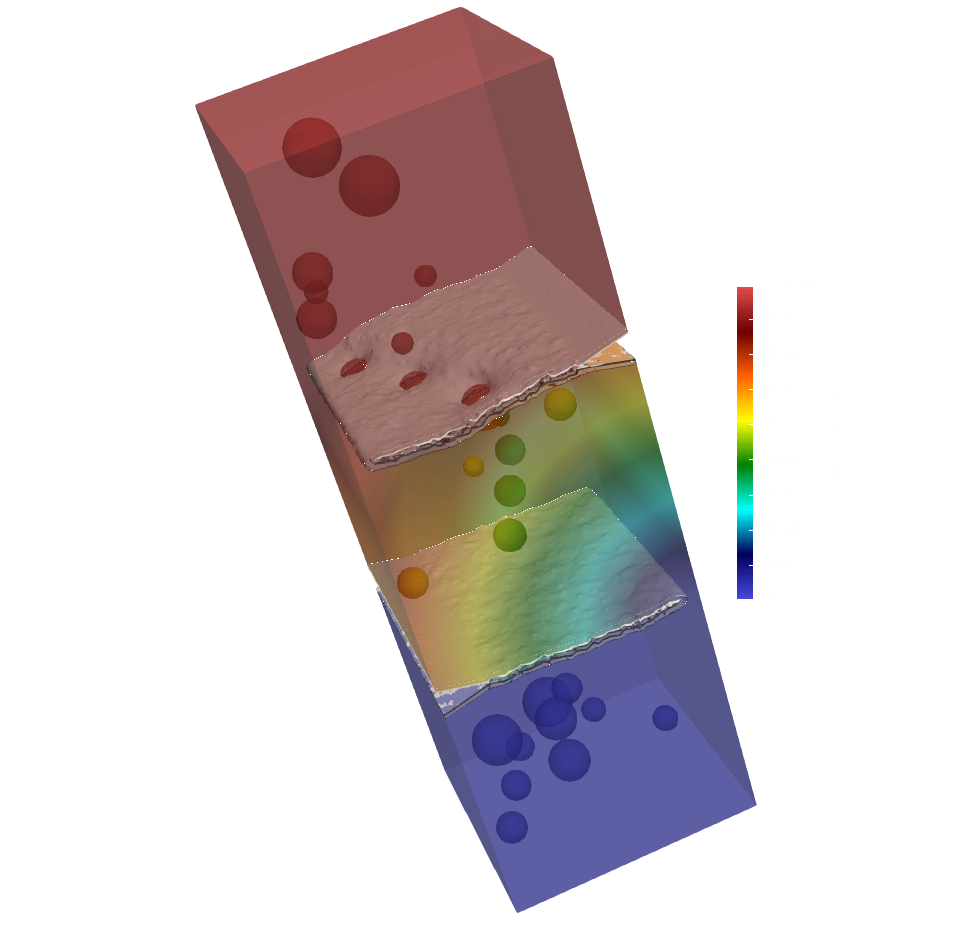
\includegraphics[width=0.45\textwidth]{rainbow-test1.png}
    \caption{Perforated concrete bar cracking.}
    \label{fig:rainbow}
\end{figure}

\begin{figure}
    \centering
    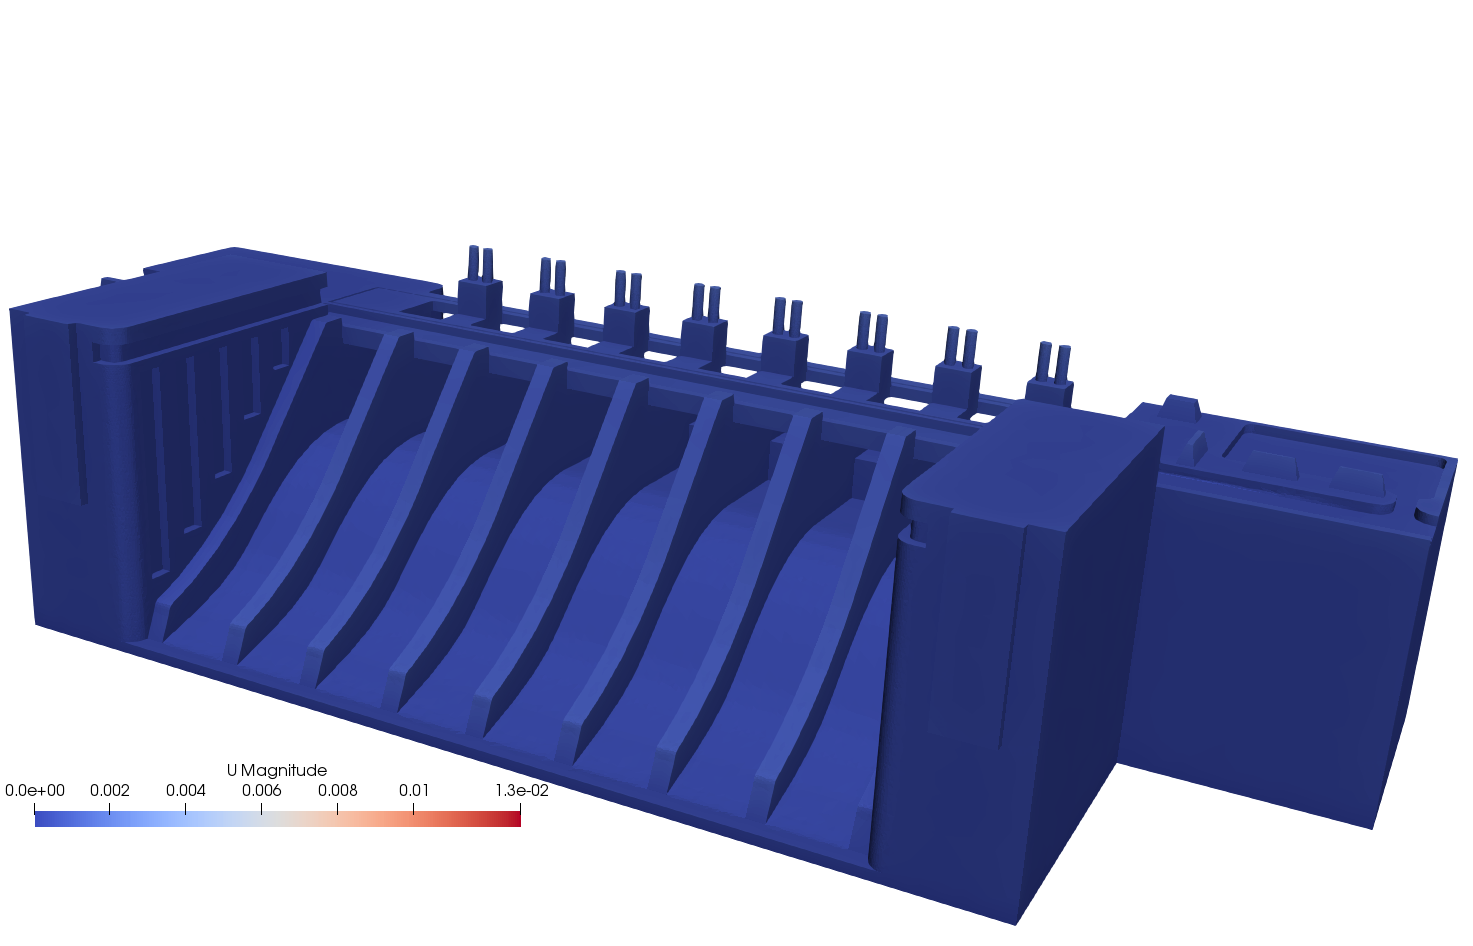
\includegraphics[width=0.45\textwidth]{dam1.png}    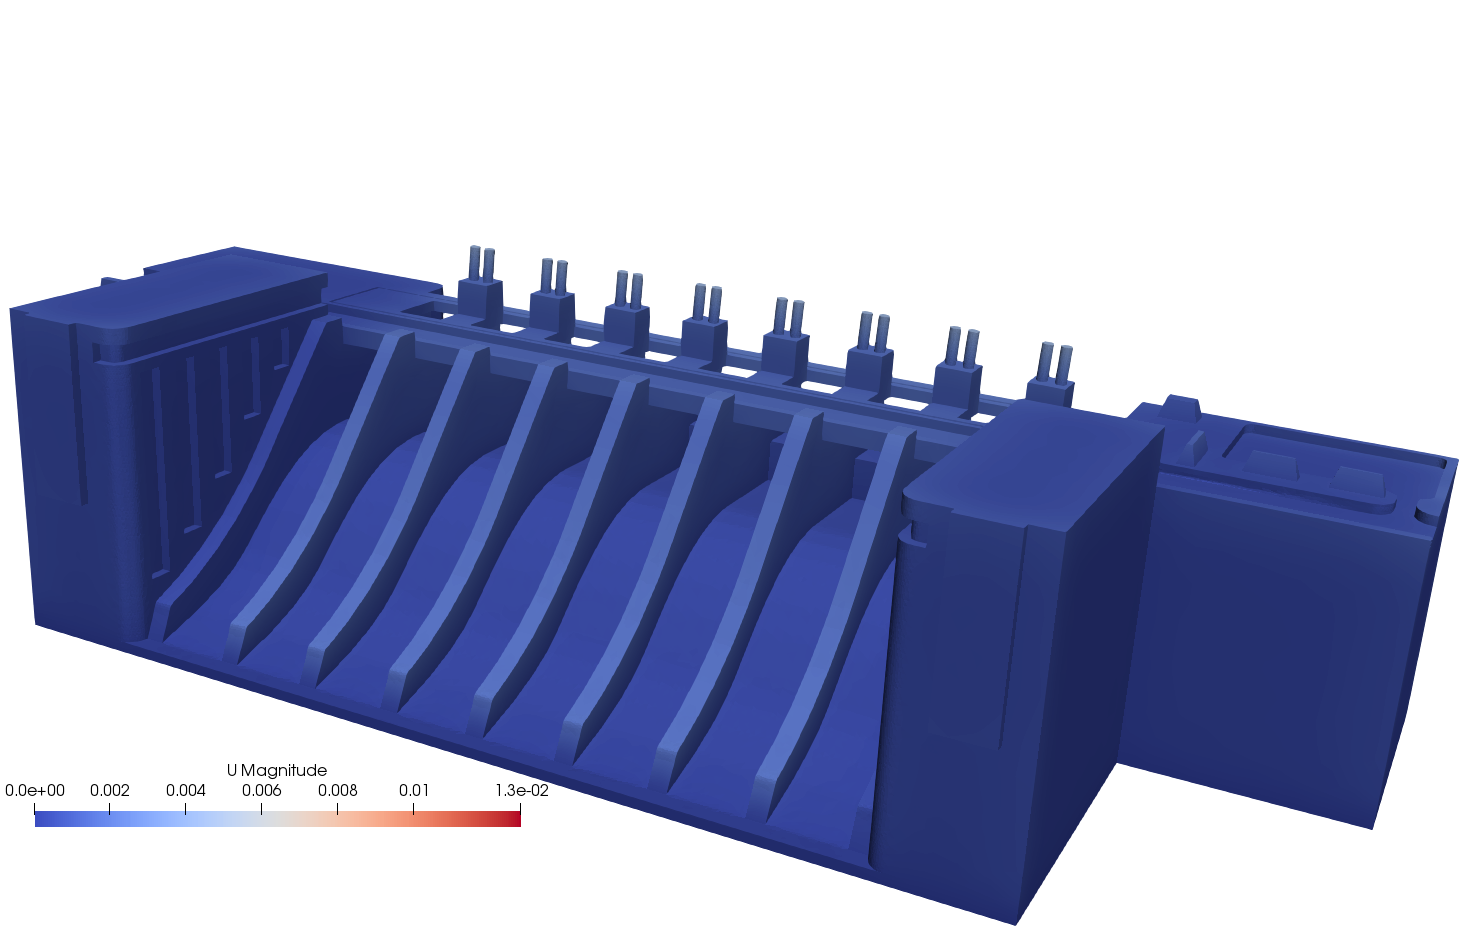
\includegraphics[width=0.45\textwidth]{dam2.png}\\
    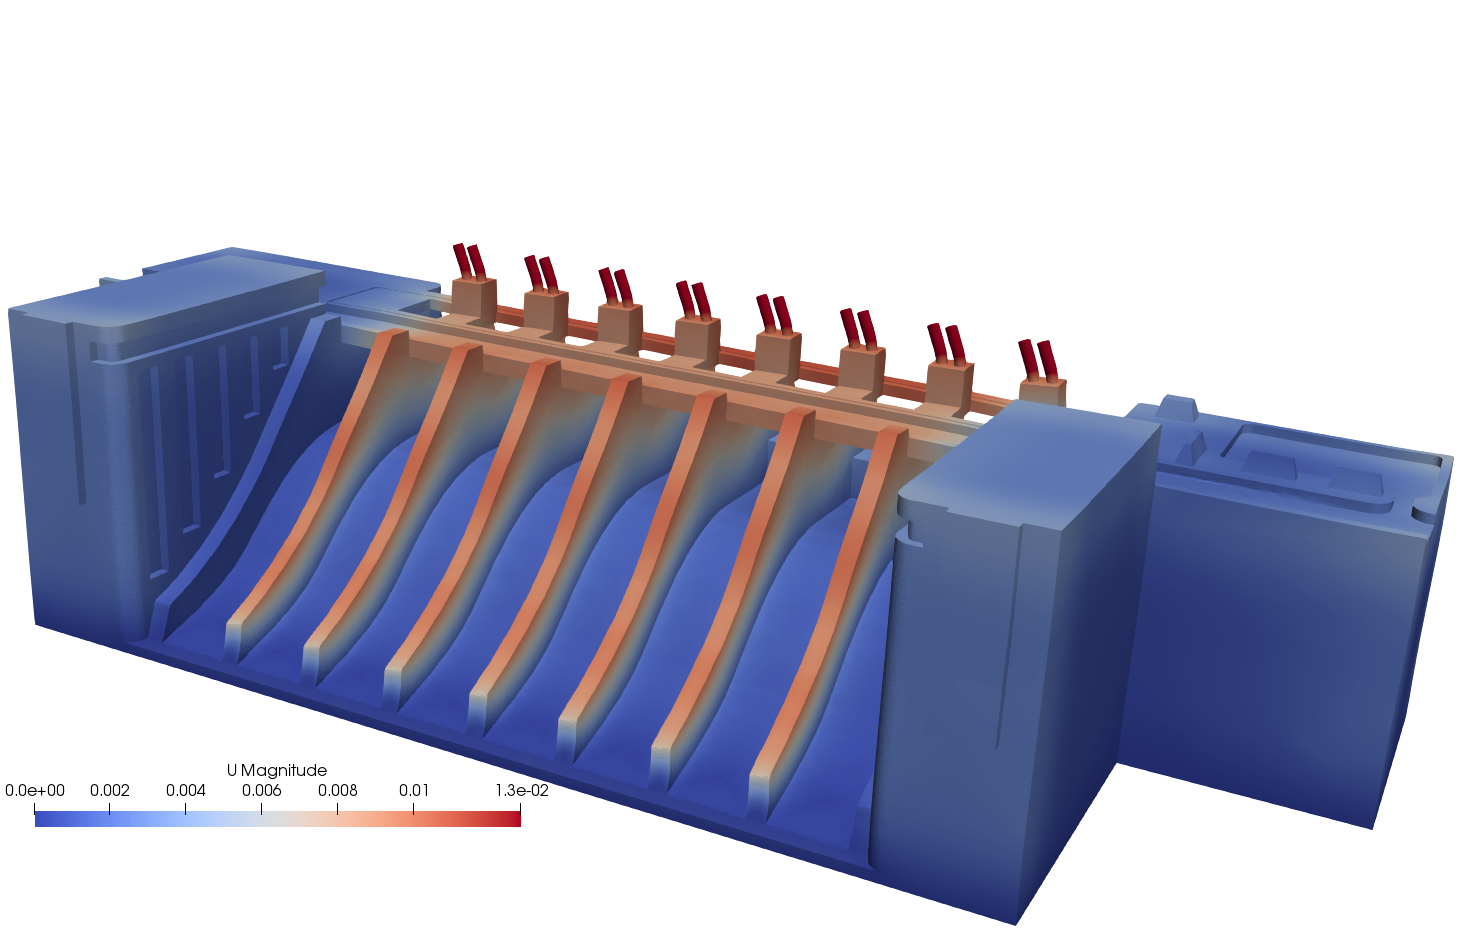
\includegraphics[width=0.45\textwidth]{dam3.png}
    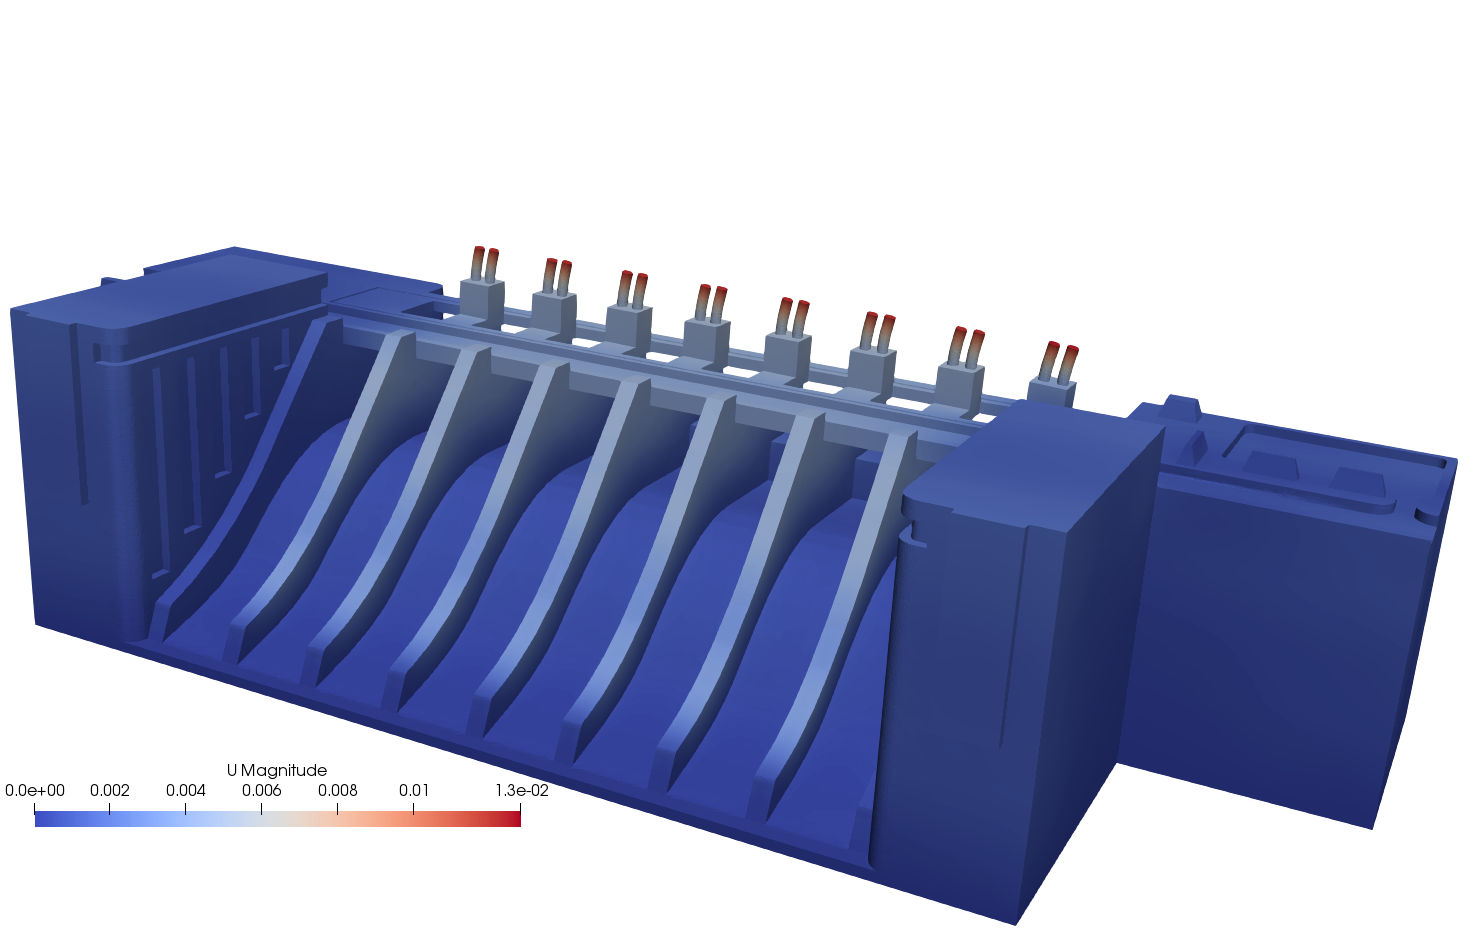
\includegraphics[width=0.45\textwidth]{dam4.png}
    \caption{Full scale dam under seismic load.}
    \label{fig:dam}
\end{figure}

\begin{figure}
    \centering
    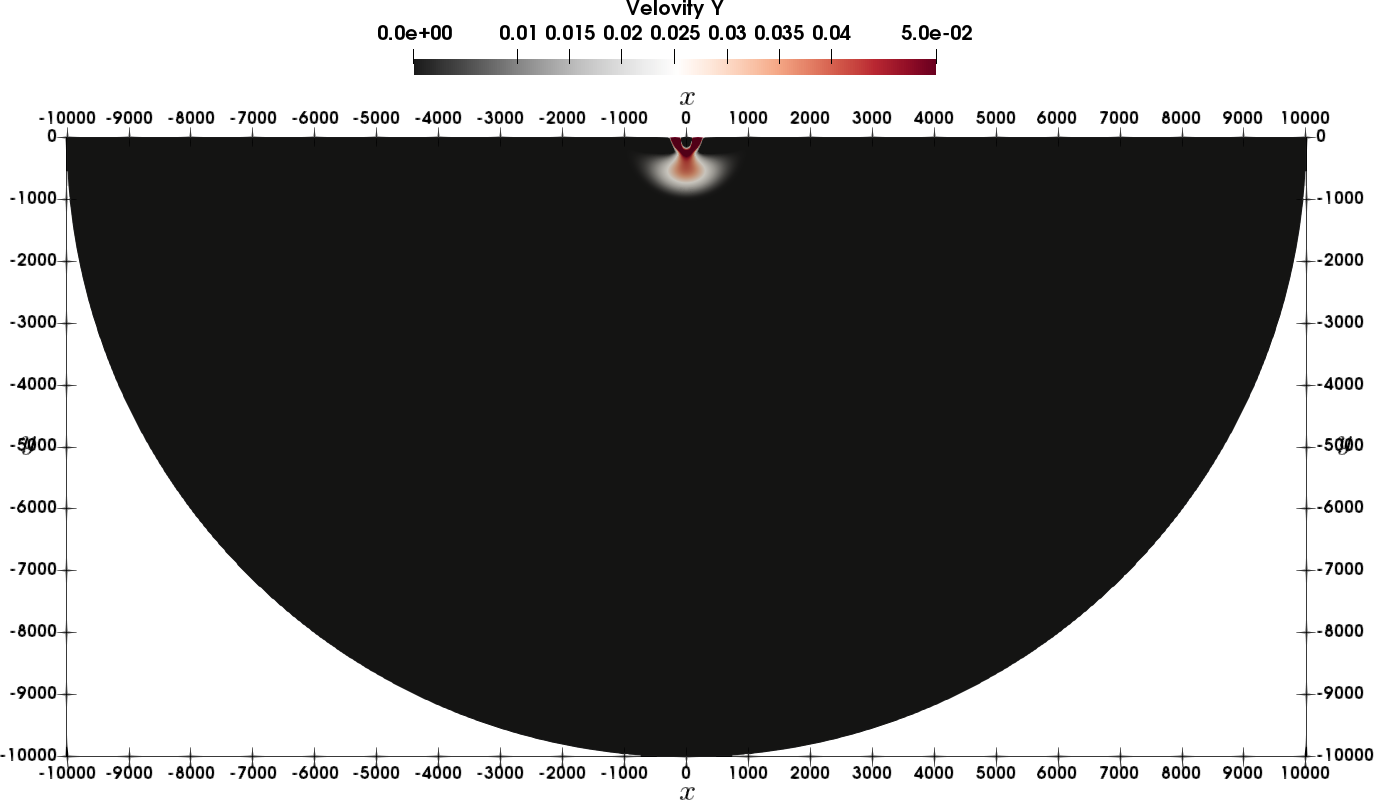
\includegraphics[width=0.3\textwidth]{t1-large.png}        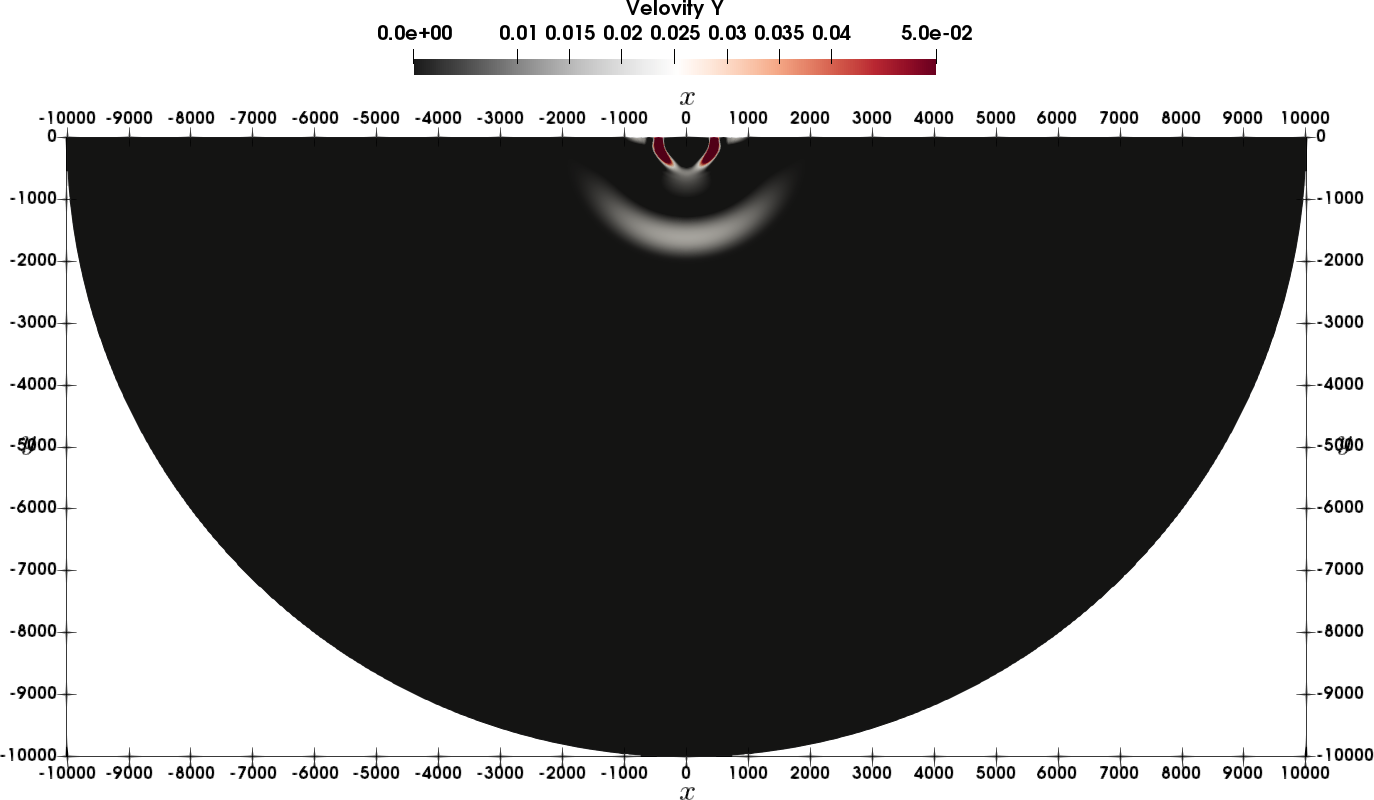
\includegraphics[width=0.3\textwidth]{t2-large.png}    
    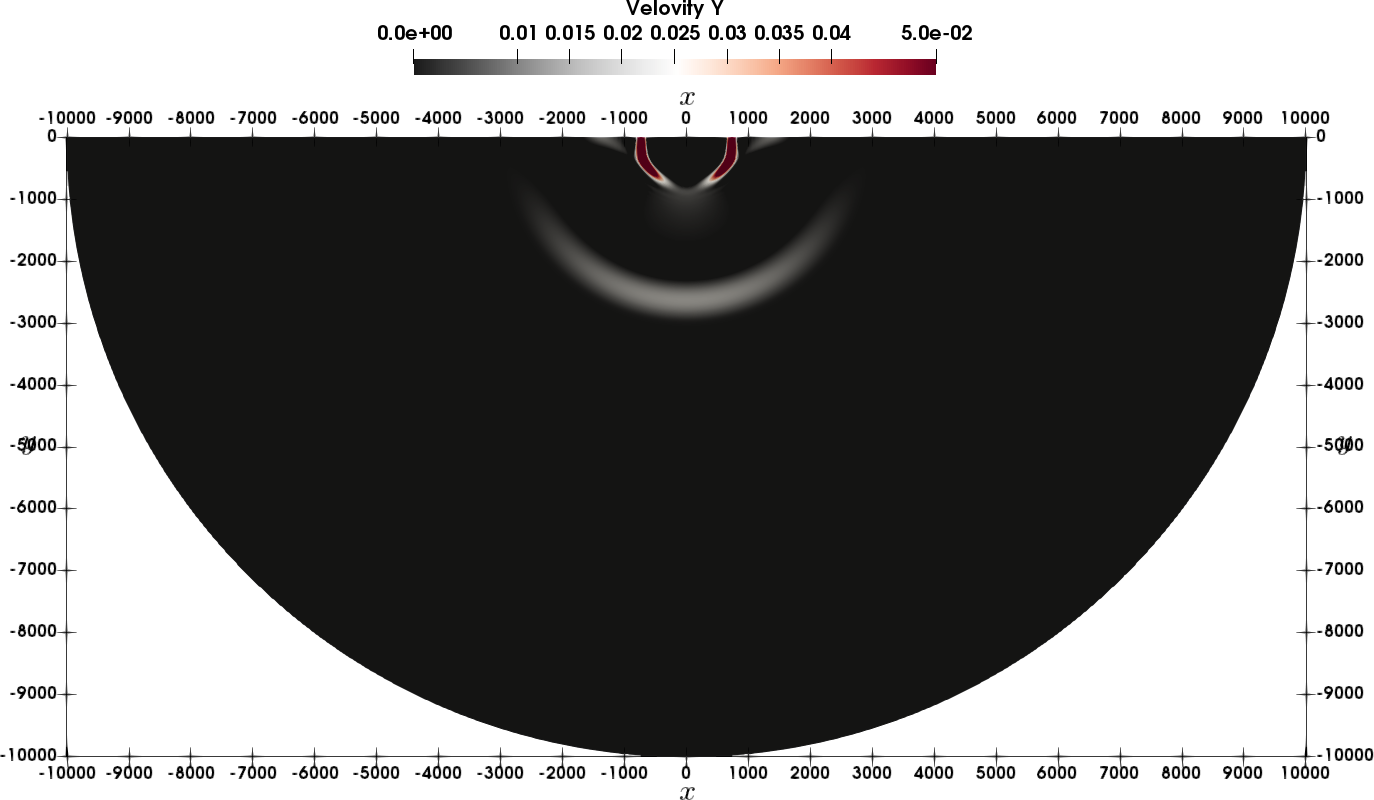
\includegraphics[width=0.3\textwidth]{t3-large.png}\\
    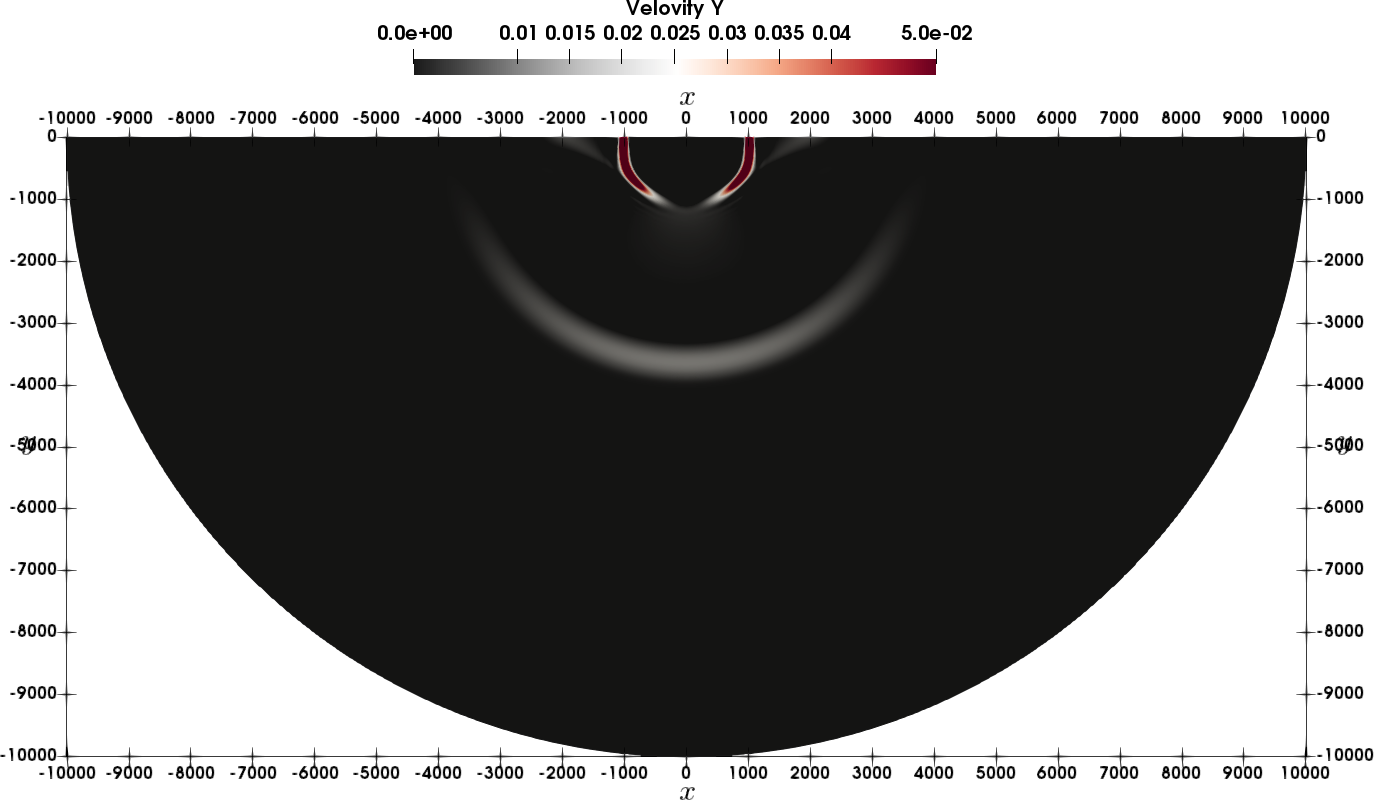
\includegraphics[width=0.3\textwidth]{t5-large.png}        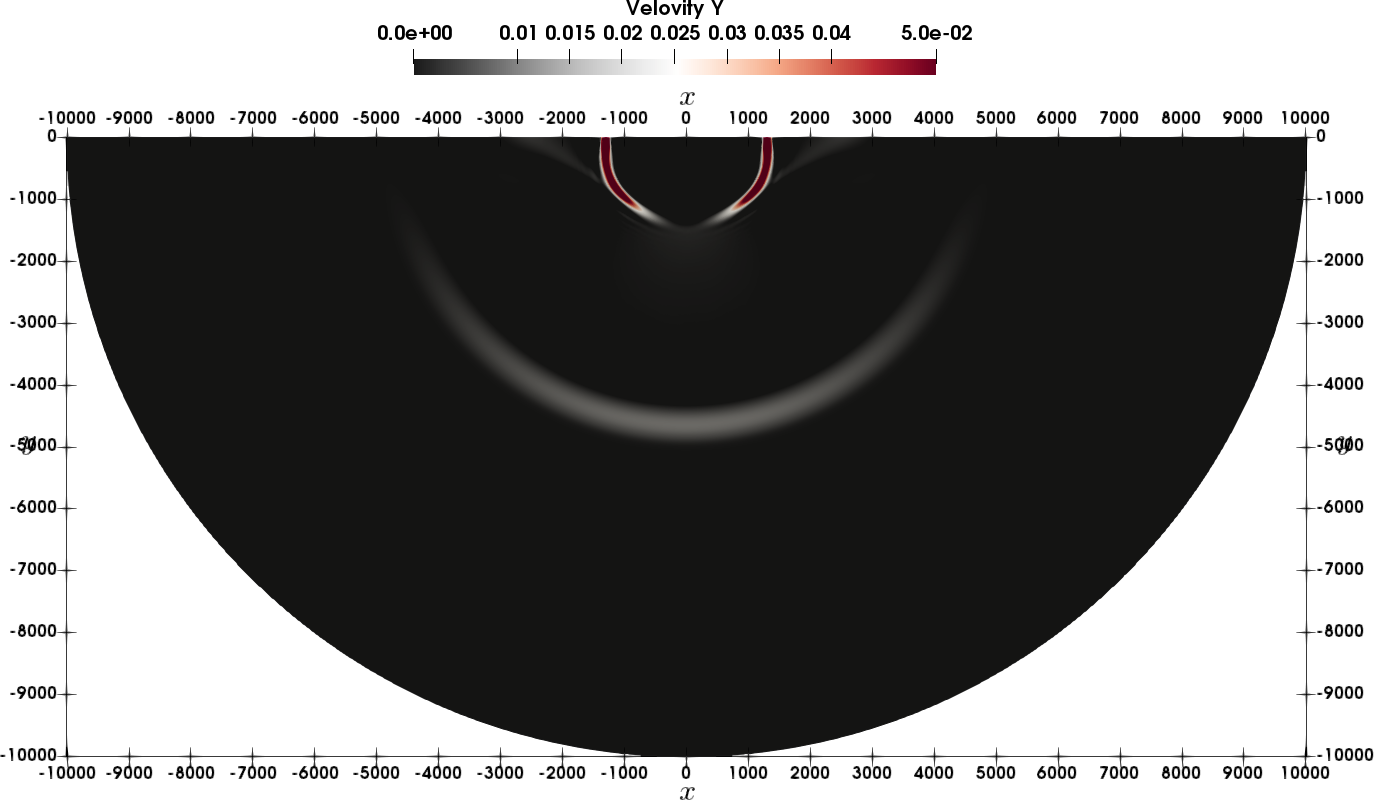
\includegraphics[width=0.3\textwidth]{t6-large.png}    
    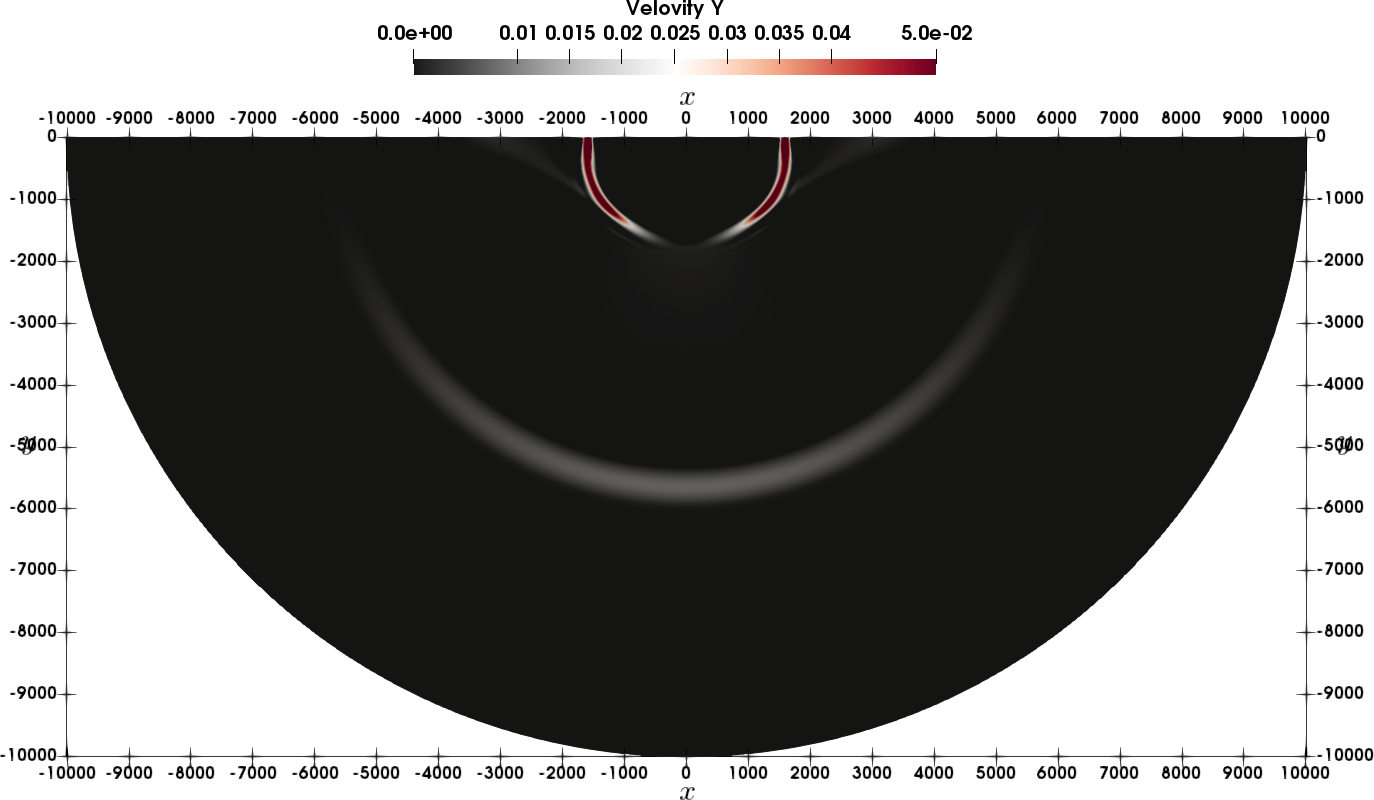
\includegraphics[width=0.3\textwidth]{t7-large.png}\\
    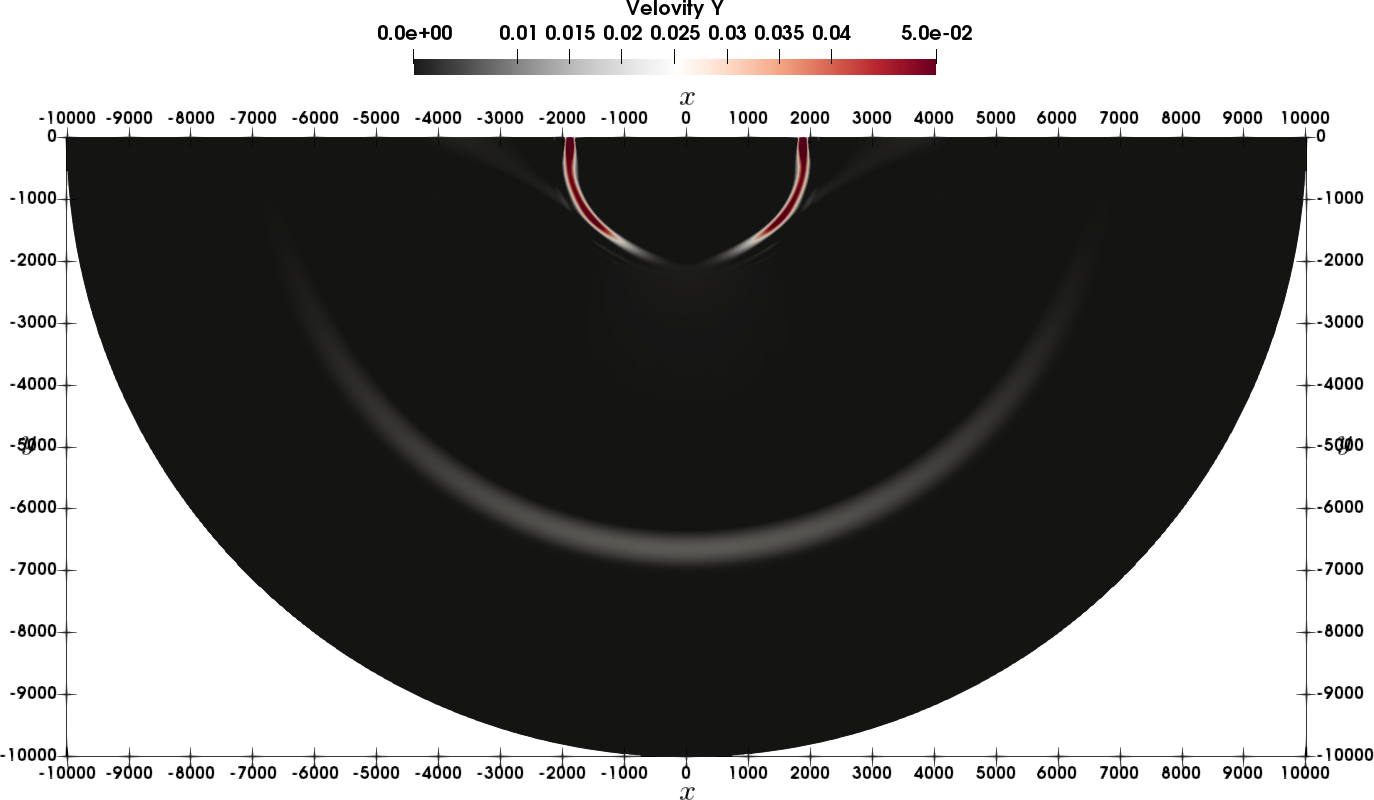
\includegraphics[width=0.3\textwidth]{t8-large.png}        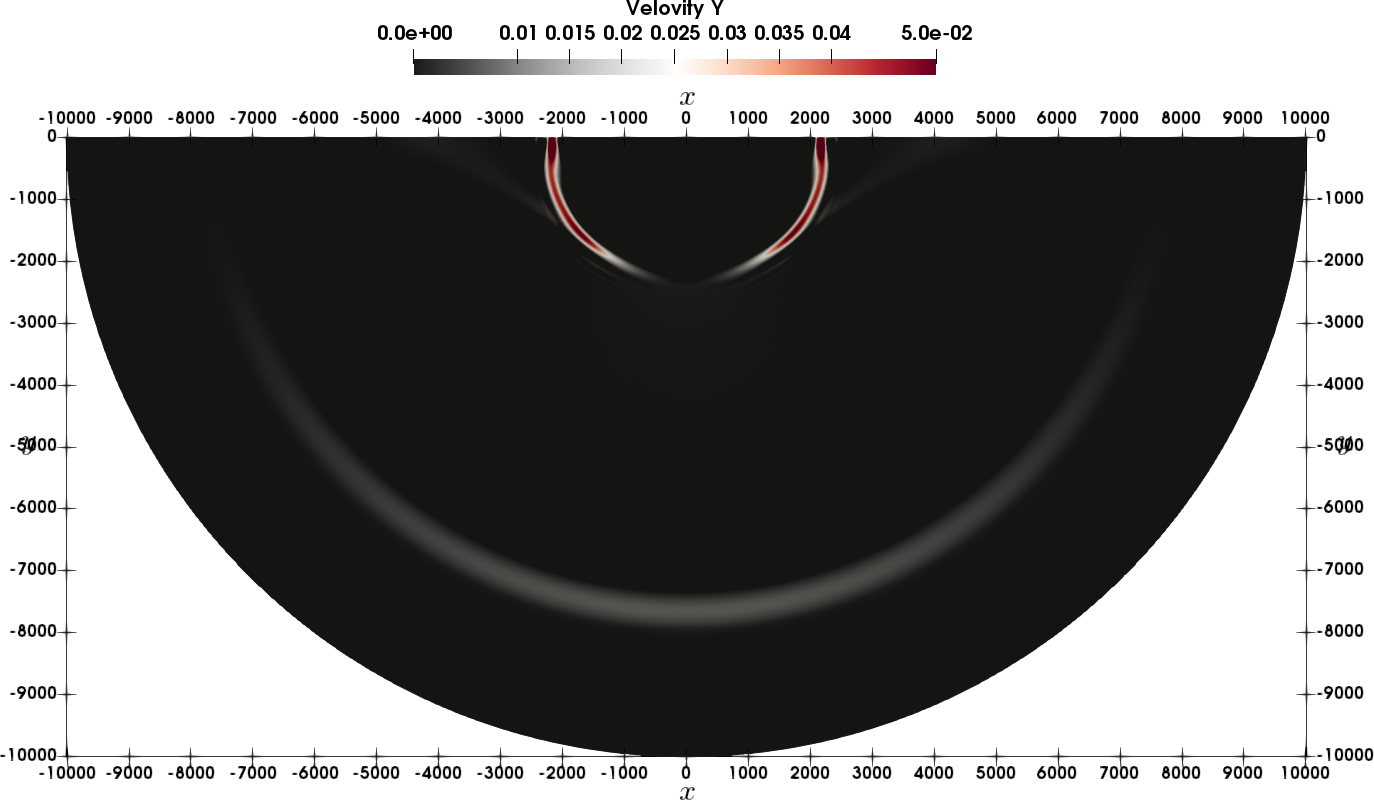
\includegraphics[width=0.3\textwidth]{t9-large.png}    
    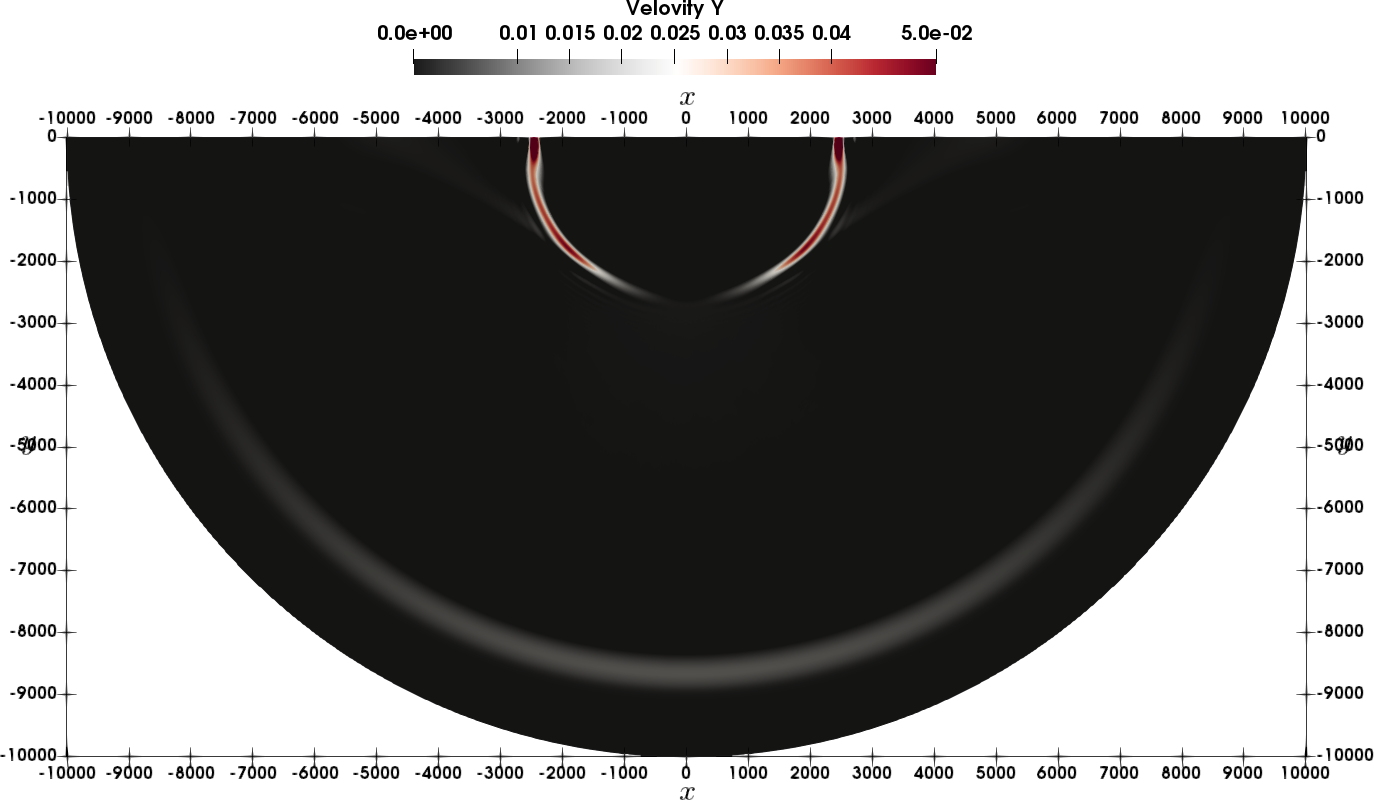
\includegraphics[width=0.3\textwidth]{t10-large.png}\\
    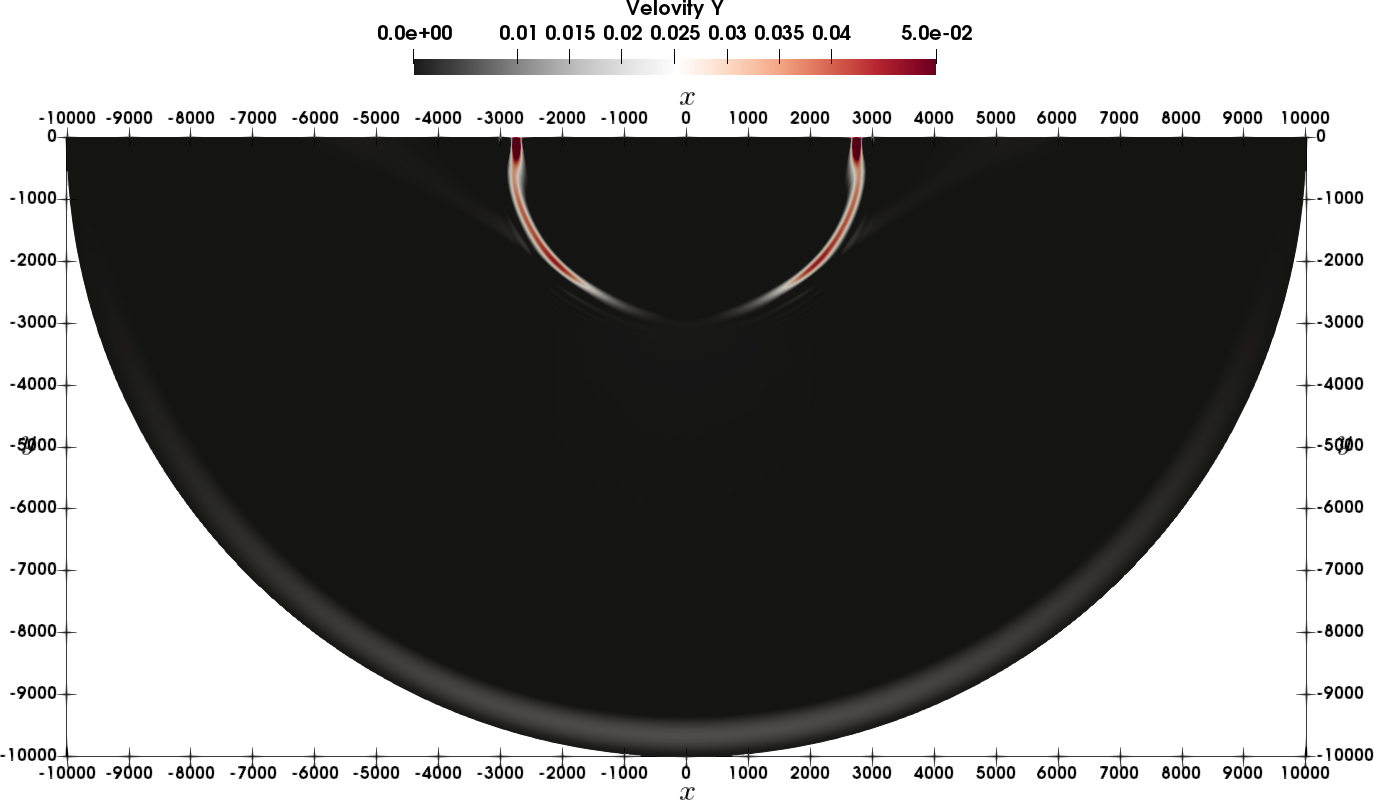
\includegraphics[width=0.3\textwidth]{t11-large.png}        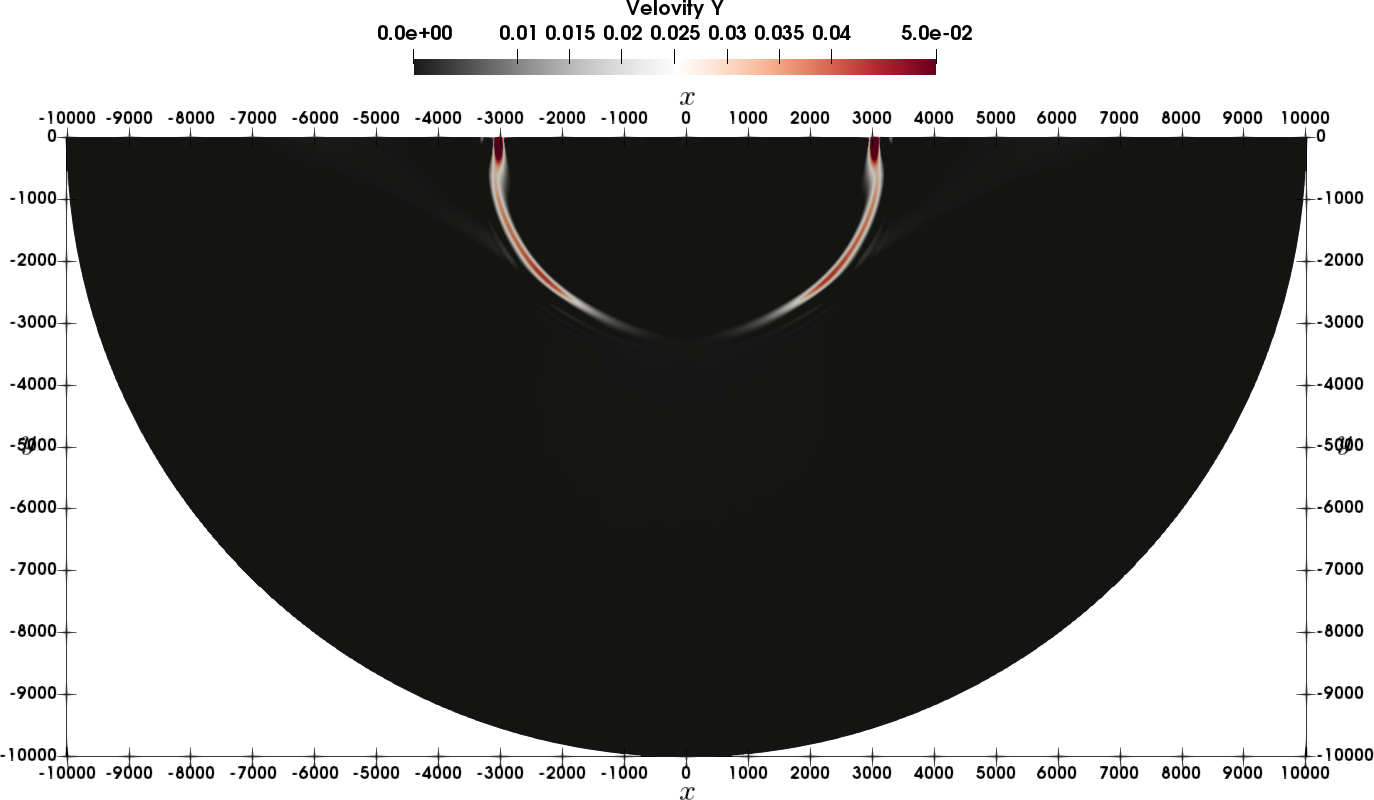
\includegraphics[width=0.3\textwidth]{t12-large.png}    
    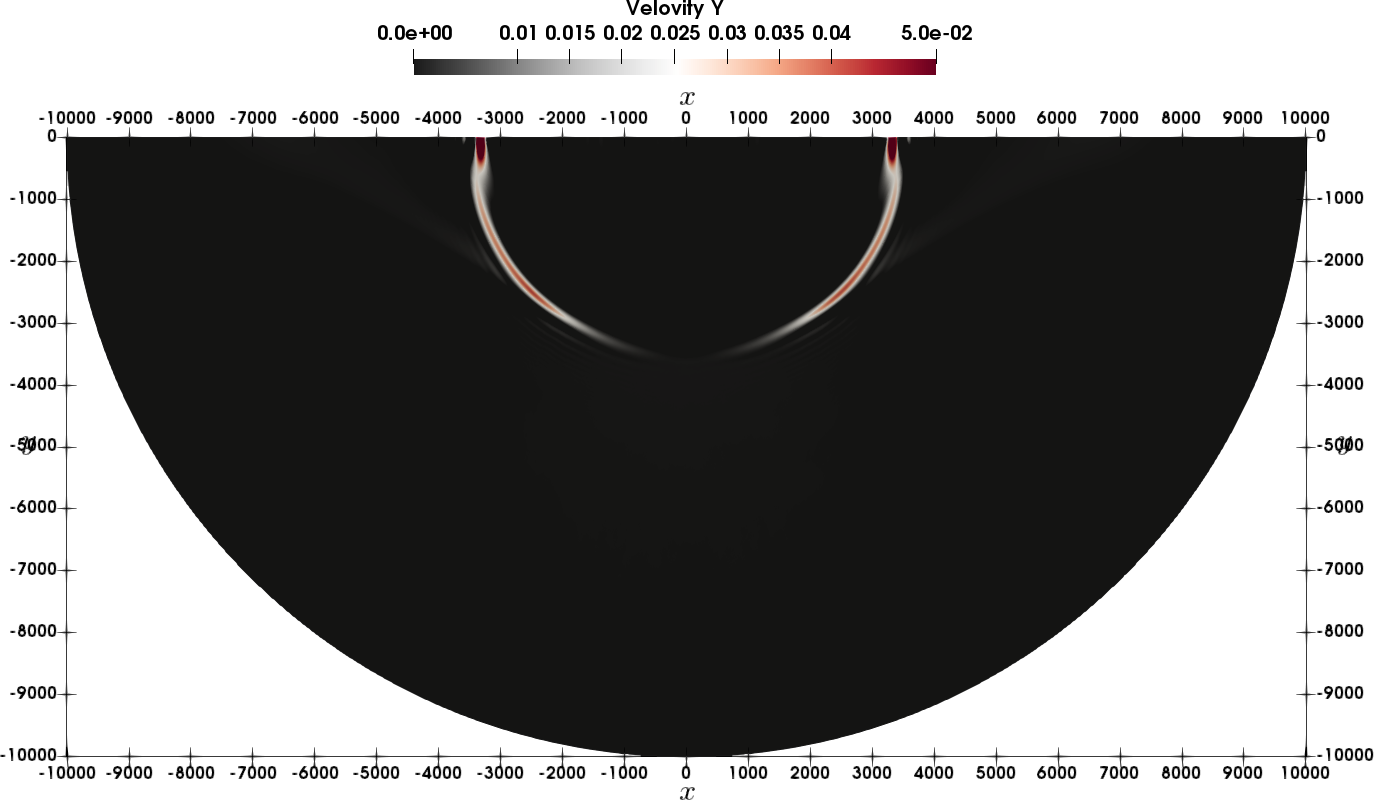
\includegraphics[width=0.3\textwidth]{t13-large.png}
    \caption{Seismic signal dispersion in soil.}
    \label{fig:soilsemi}
\end{figure}


\begin{figure}
    \centering
    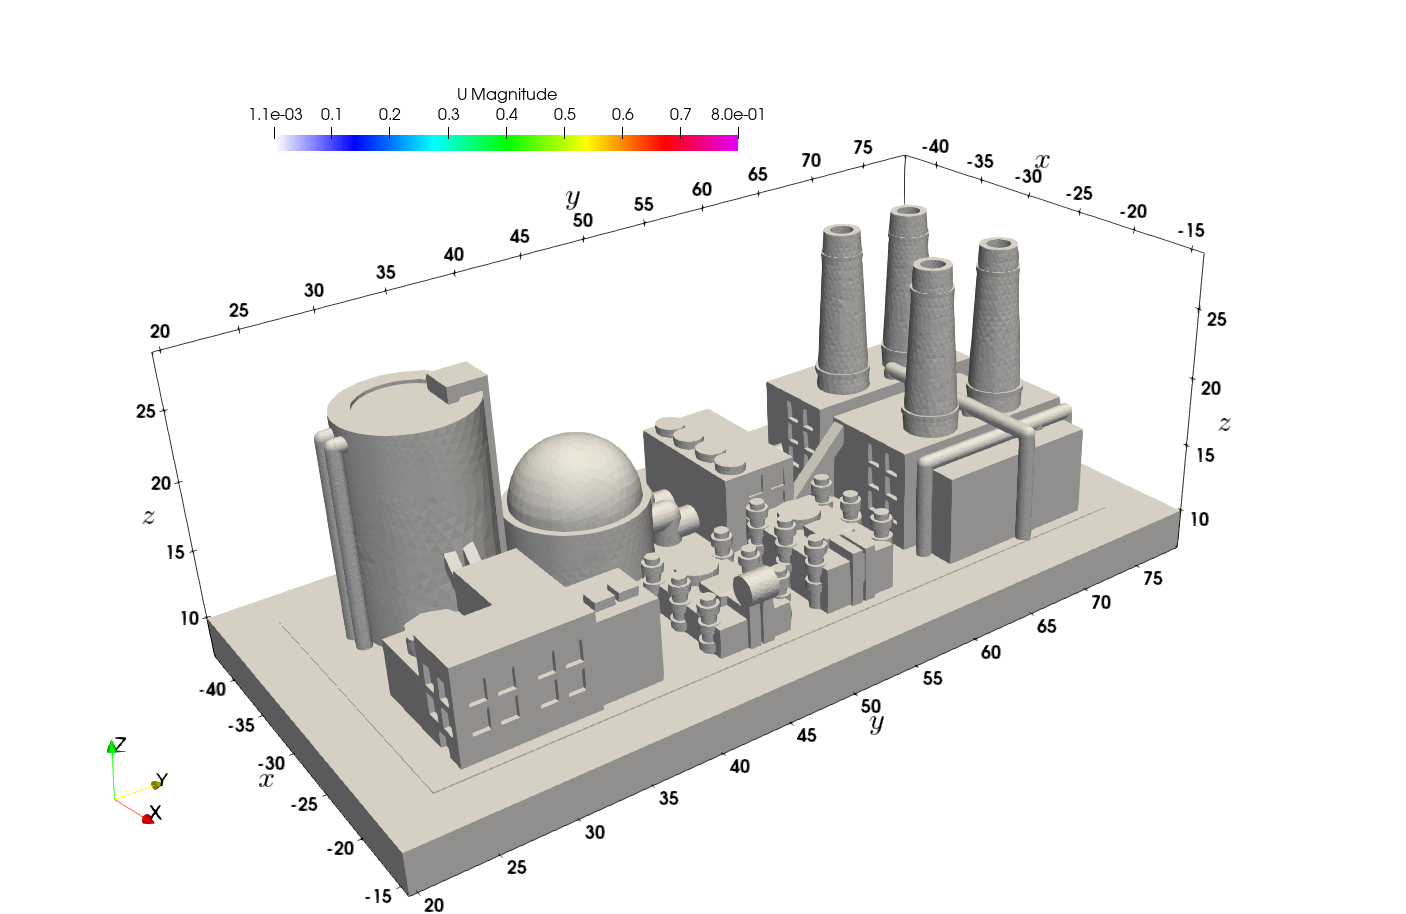
\includegraphics[width=0.65\textwidth]{t001.png}        
    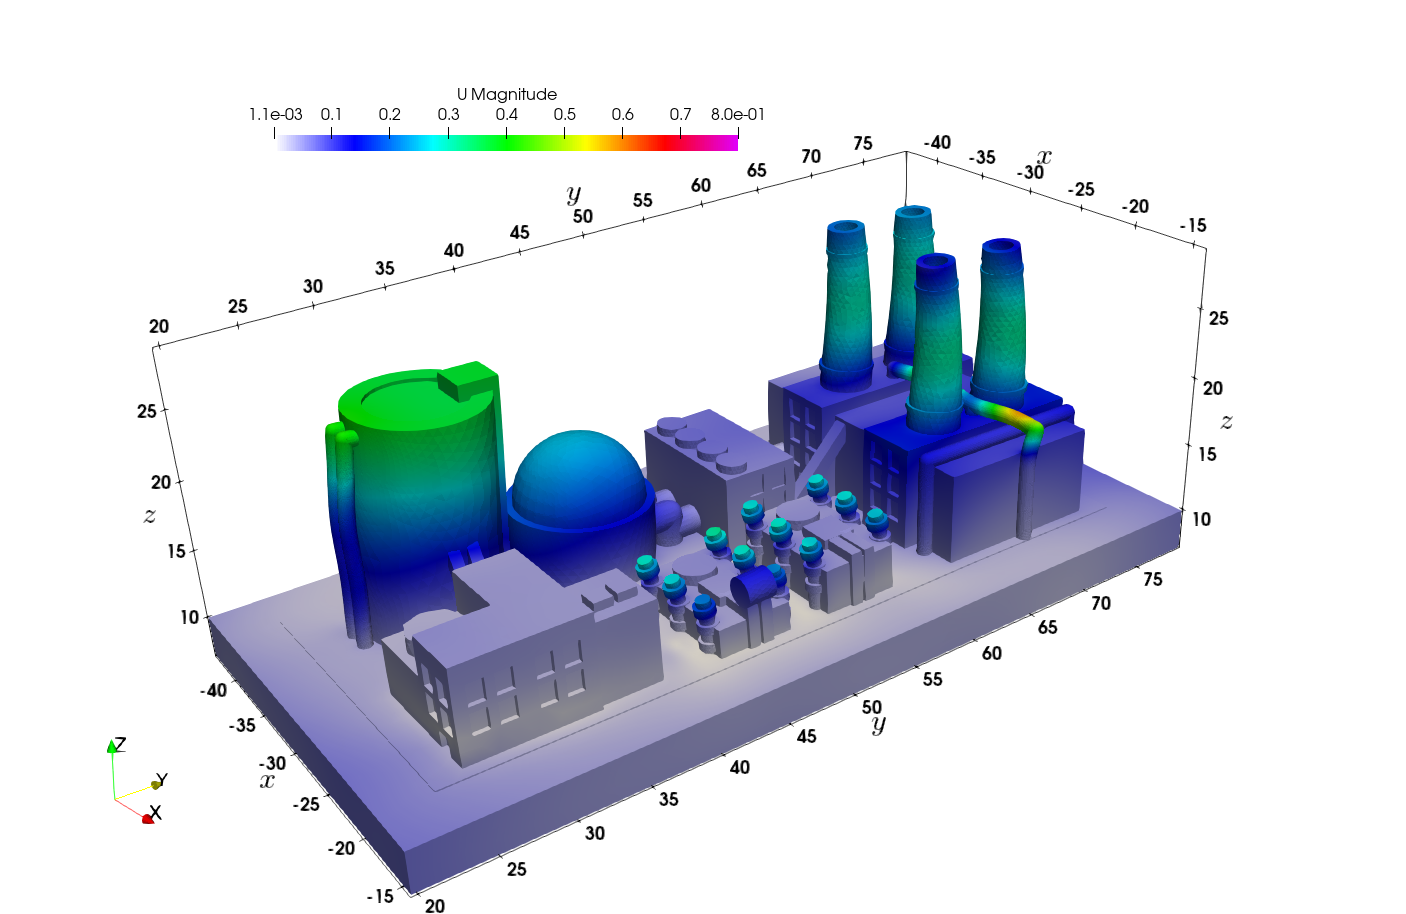
\includegraphics[width=0.65\textwidth]{t100.png}    
    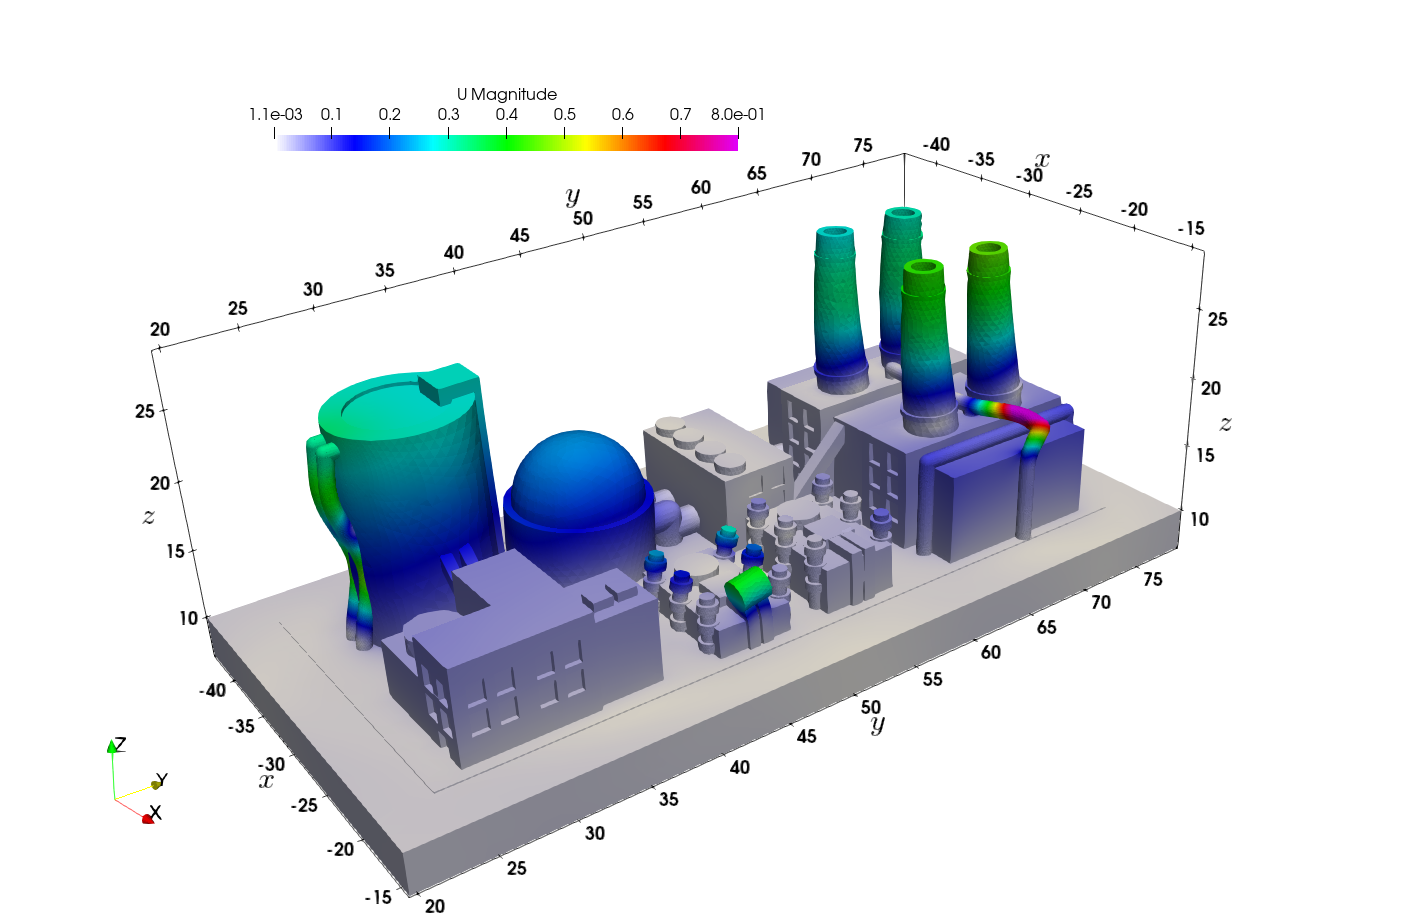
\includegraphics[width=0.65\textwidth]{t199.png} 
    \caption{Seismic signal on nuclear site.}
    \label{fig:nuclearplant}
\end{figure}

\printbibliography


\end{document}